% SPDX-License-Identifier: Apache-2.0
%
% The second TxHDL article: embedding the language in Rust.
% Built by //docs:embedding. See docs/document-build-plan.md.
\documentclass[journal,9pt]{IEEEtran}

% Two columns: listings at 6pt fit 70 columns.
\newcommand{\listingsize}{\fontsize{6}{7}\selectfont}
% SPDX-License-Identifier: Apache-2.0
%
% The house preamble, shared by every document in this directory. Loaded
% after \documentclass, before \title. Keeping it in one file is what
% stops two articles drifting apart in font, listing style or figure
% style.
% Computer Modern. IEEEtran selects Times (ptm) by default, so the face has
% to be chosen explicitly.
%
% Latin Modern is the Computer Modern variety used here, and the choice is
% forced rather than aesthetic. Under T1 encoding, plain `cmr` has no Type 1
% outlines unless cm-super is installed, and it is not in the pinned
% distribution, so pdflatex falls back to EC bitmaps and every glyph in the
% PDF becomes a Type 3 font. That was measured: the first build produced a
% document with 10 Type 3 fonts and no Type 1. Latin Modern is Computer
% Modern redrawn with a full T1 repertoire and real .pfb outlines, so the
% same design comes out scalable.
\usepackage[T1]{fontenc}
\usepackage[utf8]{inputenc}
\usepackage{lmodern}
% microtype is not in the pinned TeX distribution. emergencystretch alone
% keeps the two-column measure from producing overfull lines.
\setlength{\emergencystretch}{3em}

\usepackage{amsmath}
\usepackage{amssymb}
\usepackage{amsthm}
\usepackage{booktabs}
\usepackage{array}
% enumitem is not in the pinned TeX distribution; the list spacing below
% does what \setlist would have done.
\usepackage{float}
\usepackage{xcolor}
\usepackage{listings}
\usepackage{tikz}
\usetikzlibrary{arrows.meta,positioning,fit,backgrounds,calc}
\usepackage[hidelinks,bookmarks=true]{hyperref}

% Numbered, definition-style box for a rule the reader is meant to apply.
\theoremstyle{definition}
\newtheorem{rulebox}{Rule}
\newtheorem{example}{Example}

% Unnumbered asides.
\theoremstyle{remark}
\newtheorem*{tip}{Tip}
\newtheorem*{pitfall}{Pitfall}

% Tighter lists, in place of enumitem's \setlist.
\setlength{\topsep}{2pt}
\setlength{\itemsep}{1pt}
\setlength{\parsep}{0pt}

% Code in the running text. The typewriter face under T1 ligates `<<`
% and `>>` into guillemets, so a shift printed as \code{<<} came out as
% a French quotation mark (issue 571). microtype's \DisableLigatures is
% not in the pinned distribution, but the primitive it rests on is
% pdfTeX's own: \pdfnoligatures strips every ligature from the font it
% is given, and the current font inside \texttt is the typewriter face
% at the size in use, so each size is stripped the first time \code
% sets it. Code wants no ligature at all: two quotes are two quotes.
\newcommand{\code}[1]{\texttt{\ifdefined\pdfnoligatures\pdfnoligatures\font\fi #1}}
\newcommand{\term}[1]{\emph{#1}}

% Syntax highlighting. Four roles, distinguishable in colour and still
% distinguishable in greyscale, because an IEEE article gets printed: the
% keyword is the only bold role, the comment is the only italic one, and the
% two remaining roles differ in lightness as well as in hue.
\definecolor{kwblue}{RGB}{20,60,150}
\definecolor{cmtgreen}{RGB}{90,120,90}
\definecolor{strred}{RGB}{150,50,40}
\definecolor{numgray}{gray}{0.45}
\definecolor{framegray}{gray}{0.70}
\definecolor{bgshade}{gray}{0.97}
% A darker fill for figure cells. The listing background has to stay very
% light to keep code readable; a figure cell has to be clearly shaded or the
% distinction it draws is invisible in print.
\definecolor{cellshade}{gray}{0.90}

% The listing size is the document's choice, because it depends on the
% column: a two-column article sets `\listingsize` to 6pt and keeps its
% listings within 70 columns, or to 5.6pt when it includes source that
% rustfmt sets at 80, which is what fits a column's frame (issue 1061);
% a one-column document keeps the body size and includes source files
% at 80. `//docs:frame_test` checks every listing line against its frame. Lines are never broken; a line that does not fit
% overflows the frame, which is visible, rather than wrapping, which is
% not.
\providecommand{\listingsize}{\scriptsize}

% `'` is deliberately not a string delimiter: the language uses it for loop
% labels, as Rust does, so treating it as a quote would swallow the rest of
% the line.
\lstdefinestyle{txhdl}{
  basicstyle=\ttfamily\listingsize,
  keywordstyle=\bfseries\color{kwblue},
  commentstyle=\itshape\color{cmtgreen},
  stringstyle=\color{strred},
  numberstyle=\tiny\color{numgray},
  morekeywords={mod,use,pub,const,type,struct,enum,trait,impl,fn,async,let,mut,
    match,if,else,loop,while,for,in,break,continue,return,as,await,
    module,bus,channel,transaction,protocol,pipeline,flow,seq,config,
    port,stage,pipe,instance,connect,bind,tag,domain,blackbox,foreign,
    property,role,signal,handler,true,false,
    sequence,interface,modport,implements,package,import,var,wire,func,proc,
    case,default,next,fork,branch,join,state,fsm},
  morecomment=[l]{//},
  morestring=[b]",
  showstringspaces=false,
  columns=fullflexible,
  keepspaces=true,
  breaklines=false,
  % Framed, so a listing is bounded rather than floating in the column.
  frame=single,
  rulecolor=\color{framegray},
  framesep=3pt,
  backgroundcolor=\color{bgshade},
  xleftmargin=3pt,
  xrightmargin=3pt,
  aboveskip=6pt,
  belowskip=6pt,
  % Every listing is numbered and captioned, so it can be referred to by
  % number. `caption` without `float` numbers the listing and leaves it
  % where it was written, which is what a listing in running prose needs.
  captionpos=b,
  abovecaptionskip=2pt,
  belowcaptionskip=6pt,
}

% Figures drawn as text. Framed the same way, and with the highlighting
% switched off, because a box-and-arrow diagram is not code and half its
% words turning blue reads as an accident. Setting a style adds keys rather
% than clearing the ones already set, so the three roles are neutralised by
% hand rather than by leaving them out. Program output is printed in this
% style too, and a netlist's assignment can run past the frame, so a line
% that does not fit is broken and the rest indented; source never is.
\lstdefinestyle{ascii}{
  basicstyle=\ttfamily\listingsize,
  keywordstyle=\ttfamily,
  commentstyle=\ttfamily,
  stringstyle=\ttfamily,
  columns=fullflexible,
  keepspaces=true,
  breaklines=true,
  breakindent=2em,
  frame=single,
  rulecolor=\color{framegray},
  framesep=3pt,
  backgroundcolor=\color{bgshade},
  xleftmargin=3pt,
  xrightmargin=3pt,
  aboveskip=6pt,
  belowskip=6pt,
}
\lstset{style=txhdl}

% House TikZ styles. `shorten` lives on the arrow styles rather than on each
% arrow, so every arrow in the document gets the gap, including ones added
% later. TikZ clips a path at a node's border, so without it an arrowhead
% butts against the box with no gap at all. Keep `node distance` well above
% twice the shorten, or the arrow shrinks to nothing.
\tikzset{
  box/.style={draw,rounded corners=2pt,align=center,inner sep=4pt,
              font=\footnotesize},
  boxf/.style={box,fill=bgshade},
  lbl/.style={font=\scriptsize\itshape,align=center},
  fl/.style={-{Stealth[length=4pt]},shorten >=2.5pt,shorten <=2.5pt},
  fld/.style={fl,dashed},
}


% The contents list: the class gives a section's number 2.75em, which
% a Roman numeral past thirty overruns onto the title, so the box is
% wider here, and a subsection's entry starts where a title does.
\makeatletter
\def\l@section#1#2{\addpenalty{\@secpenalty}\addvspace{1.0em plus 1pt}%
    \@tempdima 5.75em \begingroup \parindent \z@ \rightskip \@pnumwidth%
    \parfillskip-\@pnumwidth {\bfseries\leavevmode #1}\hfil\hbox to\@pnumwidth{\hss #2}\par%
    \endgroup}
\def\l@subsection{\@dottedtocline{2}{5.75em}{5em}}
\def\l@subsubsection{\@dottedtocline{3}{10.75em}{5.5em}}
\makeatother


\InputIfFileExists{buildstamp.tex}{}{}
\providecommand{\buildstamp}{Draft build (outside the Bazel flow).}

\title{Deleting a Language: Embedding TxHDL in Rust}

\author{Filip Filmar and Dragiša Janković%
\thanks{Both authors are independent. Filip Filmar is the
corresponding author, at f@hdlfactory.com; Dragiša Janković is
reached at linkedin.com/in/dragisa-jankovic.}%
\thanks{This article follows the TxHDL merge reported in the companion
paper. It asks what remains of the language once every construct Rust
already provides is removed. Every claim about Rust in it was compiled;
the probes are in the project repository under
\code{experiments/rust\_embedding}. The runtime library the article
describes and the examples written against it are two further
documents~\cite{runtime,examples}; the cover document~\cite{cover}
lists them all.}%
\thanks{The authors used a large language model, Claude, as an
assistant in exploring the concepts and in writing and constructing
the documents and the programs; every commit of the repository says
so and records the prompts that led to it, verbatim.}%
\thanks{\buildstamp}}

\markboth{TxHDL Embedded in Rust}{Filmar and Janković: Deleting a Language}

\begin{document}
\maketitle

\begin{abstract}
A companion paper merged two hardware description languages into one and
gave the result a Rust-shaped syntax. This paper asks the next question: if
the syntax is already Rust, why is there a separate language at all. We
remove every construct that Rust provides and keep only what is left. Of
the twenty non-Rust constructs in the merged specification, seventeen go.
Two results are worth the exercise on their own. The rule that a timeless
body may not count cycles needs no enforcement, because a cycle count is
spelled \code{.await} and a plain \code{fn} has none. And a pipeline, a
sequence and a set of parallel processes are one construct, an \code{async
fn}, differing only in how they are driven; the live-range analysis that a
\code{pipe} declaration existed to feed is what an async state machine does
already. Every claim here was compiled rather than argued, one probe a question,
and four of those compilations changed the design. Arbitrary-width
arithmetic needs nightly Rust. A unit's parallel processes cannot take
\code{\&mut self}. A \code{macro\_rules!} conditional cannot reach inside
a block, which is the strongest argument for elaborating through a
procedural macro. And one driver per wire turns out to be free: a signal
yields its two ends separately, the driving end is not \code{Clone}, so
the oldest error message in hardware design arrives as a move error. One
wall stands for an elaborator, and it is the reason the merged language
was designed with its own parser: \code{if} on a signal cannot work when a
signal has no value while the program runs. It does not stand here,
because this runtime runs the design, so a condition has a value, and
the lowering reads Rust's \code{if} and \code{match} as written. Half
of the result is Chisel's architecture in Rust, and is presented as
such. The other half, sequencing through \code{async}, is the
contribution, its nearest ancestors are Calyx and Filament rather than
Chisel, and it lowers: a process of several waits to a state machine,
a \code{for} that waits to a counted loop, and an \code{async fn} to a
pipeline. The paper closes with the experiment that showed it.
\end{abstract}

\begin{IEEEkeywords}
Hardware description languages, embedded domain-specific languages, Rust,
high-level synthesis, async, language design.
\end{IEEEkeywords}

{\footnotesize\tableofcontents}

% SPDX-License-Identifier: Apache-2.0
\section{Introduction}
\label{sec:e-intro}

\IEEEPARstart{A}{} companion paper~\cite{merge} took two hardware
description languages that had been developed independently for one
project, showed that they did not compete, and merged them. LHDL described
dataflow and left time to the compiler. TxHDL described transactions over
buses and let a module block for as many cycles as a protocol took. Four
questions needed a decision about meaning, and the analysis behind
them~\cite{unification} resolved all four.

The merged language was then given a surface syntax biased toward
Rust~\cite{syntax}, construct by construct, because Rust is familiar and
because following it removed six defects that the two sources had rather
than restating them.

This paper asks the question that arrangement invites. If the syntax is
already Rust, why is there a separate language at all?

\subsection{The experiment}

Take the merged specification and delete every construct that Rust already
provides. Rename every construct whose name collides with a Rust concept,
so that nothing means two things. Keep what is left, and see how small it
is.

The answer is that seventeen of the twenty non-Rust constructs go, and what
remains is a library rather than a keyword list.

Two of the deletions pay for the exercise on their own, and
Sections~\ref{sec:e-time} and~\ref{sec:e-pipeline} state them. A third
result is negative and matters as much: Section~\ref{sec:e-walls} gives the
one thing an embedded language cannot do, which is the thing a separate
parser was buying.

\subsection{What here is Chisel, and what is not}

Half of this paper rebuilds Chisel~\cite{bachrach2012} in Rust, and it
should say so before the reader works it out. A unit as a struct,
interfaces with directed roles, \code{mux} and \code{with!}, generators
through host-language parameters, and elaboration by running the program:
that is Chisel's architecture, and Sections~\ref{sec:e-units}
to~\ref{sec:e-binding} restate it. What Rust adds there is that one
driver per wire becomes a compile-time move error where Chisel raises an
elaboration-time exception. That is a better error, earlier, and not a
different design.

The other half is not Chisel. Chisel has no \code{async}, no
\code{await} and no sequencing; every multi-cycle protocol in it is a
state machine written by hand, which is the thing both source languages
existed to remove. Sections~\ref{sec:e-time} and~\ref{sec:e-pipeline},
where an \code{async fn} is a sequence, a pipeline and a process
according to how it is driven, and where an operator's latency is the
mapping's decision rather than the designer's, are the contribution.
Their nearest ancestors are XLS~\cite{xls}, whose DSLX is a
Rust-shaped language that the compiler schedules into pipelines, and
Calyx~\cite{calyx} and Filament~\cite{filament}, not Chisel;
Section~\ref{sec:e-related} places them, and says why XLS is also the
counterexample.

That half was, when this paper was first written, the half that did
not exist. Every probe type-checked; none \term{lowered} an
\code{async fn}, which is to say none translated it into the
registers, wires and control that a synthesis tool accepts. Lowering
is the compiler's word for going down the abstraction ladder, and it
is what turns a value that is alive across an \code{.await} into a
register that the source never named. Section~\ref{sec:e-next} states
the experiment that was to settle whether the contribution is real,
and what it found when it was run: an \code{async fn} lowers to a
pipeline, a unit's \code{run} loop to a module, and a RISC-V
core~\cite{vreteno} to a netlist that simulates against the trace of
its own source.

\subsection{Everything here was compiled}

The first draft of this work argued about what Rust would accept. That was
replaced. A Rust toolchain is now part of the repository's hermetic build,
and every claim in this paper is a probe that was compiled, one per
question. Section~\ref{sec:e-probes} reports what each one answered, and
keeps the ones that failed, because a failure is an answer.

Four of those compilations changed the design rather than confirming it,
and Section~\ref{sec:e-probes} gives all four. Two show the shape.
Arbitrary-width arithmetic does not work on stable Rust. A unit's parallel
processes cannot take a mutable borrow of the unit. Neither was visible
from the language reference; both were visible in ten lines of code.

% SPDX-License-Identifier: Apache-2.0
\section{The Rule, and What It Leaves}
\label{sec:e-rule}

\begin{rulebox}[The reduction]
Delete every construct Rust already provides. Rename every construct whose
name collides with a Rust concept. What remains is the library.
\end{rulebox}

The renaming clause does one job in practice. A hardware \term{module} and
a Rust \code{mod} are different things with one name, so the hardware one
becomes a \term{unit} and \code{mod} keeps its meaning as a namespace.

\subsection{The vocabulary that remains}

Four of the library's Rust modules hold everything the language still
needs. The library has others, the netlist, foreign modules, formal
checks and address and register maps, but those are what it does with
a design rather than words a design is written in.

\begin{lstlisting}[caption={The vocabulary that survives the reduction. Four Rust modules and two macros, and everything else is a plain struct, trait or function.},label={lst:vocab}]
crate::types::Transaction   // data that moves between units
crate::types::Tag           // a domain and its policy

crate::comp::Unit         // a unit
crate::comp::Bus            // a bundle of channels
crate::comp::Chan           // one channel, its ends Tx and Rx
crate::comp::Signal         // one wire, its ends Out and In
crate::comp::Clock          // a clock domain, as a type

crate::pipeline::*          // operators that may take a cycle. async,
                            // and a pipeline stage once awaited
crate::funcs::*             // operators that cannot. plain fn

interface!                  // a link's members, a struct per role
config!                     // a build, as one item
\end{lstlisting}

Everything else is a plain Rust struct, trait or function.
Table~\ref{tab:reduction} states the mapping.

\begin{table}[H]
\caption{What each construct becomes. Seventeen of twenty are deleted
outright.}
\label{tab:reduction}
\centering
\footnotesize
\begin{tabular}{@{}ll@{}}
\toprule
Was & Is now \\
\midrule
\code{transaction T}   & \code{struct T} plus \code{\#[derive(Transaction)]} \\
\code{module M}        & \code{struct M}, a unit, plus \code{impl Unit} \\
\code{bus B}           & \code{struct B} plus \code{\#[derive(Bus)]} \\
\code{interface I}     & \code{interface!}, its members declared once \\
\code{modport R}       & \code{struct R}, which \code{interface!} writes \\
\code{channel c: T}    & a field of type \code{Chan<T>} \\
\code{port p}          & an end the unit's \code{run} takes \\
\code{flow f}          & \code{fn f} \\
\code{seq s}           & \code{async fn} \\
\code{pipeline stage pipe} & \code{async fn} and \code{.await} \\
\code{tag T}           & \code{struct T} plus \code{impl Tag}, as a parameter \\
\code{config bind}     & a \code{type} alias \\
\code{domain D}        & a type parameter \\
\code{assert assume cover} & Rust's own macros \\
\bottomrule
\end{tabular}
\end{table}

\subsection{Transactions, interfaces and modports}

A transaction is a struct that implements a marker trait. Nothing else
about it is special.

\begin{lstlisting}[caption={A transaction is a struct and a derive. Nothing else about it is special.},label={lst:transaction}]
#[derive(Transaction)]
pub struct MacRequest {
    pub addr: u32,
    pub count: u8,
}
\end{lstlisting}

An \code{impl} may legally precede the \code{struct} it is for, because
items in a Rust module are not order dependent, and writing
\code{impl Transaction for MacRequest} above the struct would put the kind
before the data the way \code{transaction MacRequest \{ .. \}} used to.
The derive reads the same way and stays idiomatic. It also scales, because
a struct collects several markers before long, and it has somewhere to
grow: the layout type that Section~\ref{sec:e-costs} needs for structural
compatibility is work for this derive to do later.

An interface splits into two kinds of Rust item, and that split fixes a
defect the earlier analysis reported~\cite{unification}. LHDL's
\code{interface} did two jobs at once, a bundle of wires and a socket an
implementation fills, which is why its grammar and its examples never
agreed. Here \code{interface!} declares the members once, and writes a
struct per role whose fields are the ends that role holds: a driving end
for a member it sends on, a reading end for one it takes. The macro
refuses a role that leaves a member out, and two roles that both drive
one member.

\lstinputlisting[caption={An interface declared once, with a struct per role: \code{Initiator}, \code{Target} and \code{Monitor} each hold the ends of the members they use. The probe that answered the question, \code{experiments/rust\_embedding/probe\_interface\_proc.rs}.},label={lst:interface}]{experiments/rust_embedding/probe_interface_proc.rs}

A unit takes a role's struct as a side of its \code{run}, and the
netlist flattens the struct into its members, under their names.

% SPDX-License-Identifier: Apache-2.0
\section{Values}
\label{sec:e-values}

Rust's integers are the wrong types for hardware, and the reason is not
width. It is that \code{u32} has no way to say that nobody has driven this
wire yet.

\code{crate::types} therefore defines its own, paralleling the primitives
rather than reusing them.

\subsection{Two values and nine}

\code{Bit} is two valued, and it is what synthesis maps. Its default is
\code{Zero}, because a synthesised register leaves reset at a defined
value.

\code{Logic} is nine valued, in the order IEEE 1164 gives
\code{std\_ulogic}. Its default is \code{U}, uninitialised, and that
difference is the whole reason the type exists.

\begin{lstlisting}[caption={The two value types. An undriven wire is \code{U}, not zero.},label={lst:bitlogic}]
pub enum Bit { Zero, One }

pub enum Logic {
    U,        // uninitialised
    X,        // forcing unknown
    Zero, One,
    Z,        // high impedance
    W,        // weak unknown
    L, H,     // weak 0, weak 1
    DontCare,
}
\end{lstlisting}

Narrowing is fallible, and that is the point. \code{Logic::to\_bit}
returns nothing for \code{U}, \code{X} or \code{Z}, so a design that turns
an unknown into a number has to say so rather than do it quietly.

\subsection{Resolution, not a rule of our own}

Two drivers on one wire are resolved by the IEEE 1164 table, which the
library implements rather than paraphrases.

\begin{lstlisting}[caption={Resolution. Contention gives \code{X}; a pull-up against high impedance gives \code{H}.},label={lst:resolve}]
Logic::One.resolve(Logic::Zero)   // X
Logic::Z.resolve(Logic::H)        // H
\end{lstlisting}

Reusing the standard table costs nothing and means an engineer who knows
VHDL already knows what this does.

\subsection{Numbers}

\code{U<N>} and \code{I<N>} are the numeric vectors, and
\code{logic::Vec<N>} is a vector of \code{Logic} for when unknowns must
propagate. It lives in its own module so that the type is just
\code{Vec}: \code{logic::Vec<8>} says what it is without repeating the
word, and \code{std::vec::Vec} is untouched, because nothing is imported
unqualified. Converting between them is where the two worlds meet:
\code{logic::Vec::to\_u} returns nothing unless every bit is defined.

\begin{lstlisting}[caption={An undriven vector is unknown, and says so.},label={lst:undriven}]
let v = logic::Vec::<8>::default();   // eight U's
assert!(v.to_u().is_none());
\end{lstlisting}

Same-width arithmetic, resizing to a stated width and slicing all compile
on stable, because each result width is a standalone const parameter. So
does a multiply whose result width is \emph{stated}, \code{a.mul::<64>(b)},
because \code{64} is standalone too. What does not compile is a multiply
whose result width is \emph{computed}, \code{U<\{A + B\}>}, for the
reason Section~\ref{sec:e-probes} gives: that is the one thing stable
Rust will not accept, so the width is written by the caller rather than
derived.

A number is written as a number. \code{U<N>} converts from every unsigned
primitive and from \code{i32}, and its operators and every drive take
anything that converts, so \code{acc + 1}, \code{n == 0} and
\code{reg.set(0)} say what they mean. The operators are Rust's,
\code{+}, \code{-}, \code{\&}, \code{|}, \code{\^{}}, \code{!},
\code{<<}, \code{>>} and the compares, through the \code{std::ops}
traits; a compare yields a \code{bool}, since \code{PartialEq} allows
nothing else, and a \code{bool} converts to a \code{Bit} and back, so
a condition is either. \code{i32} is there because an
integer literal with no other constraint is an \code{i32}, and a literal
is the common case; a negative one is a bug, and debug builds say so.

% SPDX-License-Identifier: Apache-2.0
\section{The Model of Time Enforces Itself}
\label{sec:e-time}

The merged specification spends a section on one rule. A timeless body may
not count cycles; a sequenced body counts them exactly as written. It gives
the two bodies two keywords, \code{flow} and \code{seq}, and states that a
cycle count inside a \code{flow} is a compile error.

Embedded in Rust, that rule needs no enforcement, because it cannot be
broken.

A cycle count is spelled \code{.await}. A plain \code{fn} is not
\code{async}, so it has no \code{.await} to write, so it cannot state a
cycle count. The compiler rejects the attempt already, with its own error
about awaiting outside an async context, and the specification says
nothing.

\begin{lstlisting}[caption={The model of time, enforced by the type system. The first function has no \code{.await} to write, so it cannot state a cycle count.},label={lst:time}]
// Timeless: combinational. There is no .await to write.
fn narrow(v: U<64>, low: bool) -> U<32> {
    mux(low, low_half(v), high_half(v))
}

// Sequenced. Counts cycles exactly as written.
async fn main(&mut self) {
    loop {
        let req = self.host.request.wait().await;
        cycles(BAUD_TICKS).await;
    }
}
\end{lstlisting}

Two constructs are deleted, and a rule that needed a paragraph of
specification and a compiler check becomes a fact about the type system.

The division is not between cheap operations and expensive ones. It is
between operations that finish inside a cycle and operations that do not.
A multiply is \code{async} for that reason, and
Section~\ref{sec:e-pipeline} shows what follows from it.

This is the clearest case of the reduction paying for itself, and it is
worth saying why it works rather than treating it as luck. The original
rule and Rust's rule are the same rule. LHDL's eighth thesis~\cite{theses}
argued that a designer should state intent and leave the mapping to time to
the implementation. Rust's \code{async} exists to mark exactly the place
where a computation gives up control and resumes later. Both are drawing
the same line, so one of them can be deleted.

% SPDX-License-Identifier: Apache-2.0
\section{A Pipeline Is an Async Function}
\label{sec:e-pipeline}

A pipeline and a sequence are one construct driven two ways.

A sequence runs one invocation to completion before starting the next. A
pipeline starts a new invocation every cycle, so several are in flight at
once, each at a different point in the body. Nothing about the body
differs. The difference is the rate at which invocations start, and that
belongs at the call site.

\begin{lstlisting}[caption={A pipeline, a sequence and a parallel process, all at once. Nobody placed the stage boundary: it is where an operator with latency is awaited.},label={lst:pipeline}]
use crate::pipeline::{add, mul};

async fn mac(a: U<32>, b: U<32>, prev: U<64>) -> U<64> {
    let p = mul(a, b).await;   // the multiplier's latency
    add(prev, p).await         // and the adder's
}
\end{lstlisting}

\subsection{Nobody places the stage boundary}

An earlier draft of this listing wrote \code{tick().await} to say where
the register goes. That was wrong, and wrong in a way the project has
already ruled on: the eighth thesis~\cite{theses} asks the language to
stop making a designer place registers by hand, and a hand-placed tick is
exactly that under a new name.

Operators that have latency are \code{async} instead, and they live in
\code{crate::pipeline}, because each of them is a pipeline stage the
moment it is awaited. Combinational operators live in
\code{crate::funcs}, so the module a design imports from already says
whether the operation can cost time. A multiply takes as long as the
mapping decides, so
\code{mul} is awaited and the caller never learns the number. An adder is
the same: \code{add} is awaited too, because whether an addition costs a
cycle is a question about the adder and the clock, not about the design.

\subsection{Why there is no \code{impl Add}}

Writing \code{prev + p} would be shorter, and it is not offered.

An operator has to return a value. An operation whose latency the mapping
decides cannot, so \code{+} could only be provided for the zero-latency
case, and a design that wrote it would have chosen a combinational adder
without saying so. The shorter spelling would be the one that quietly
makes the decision the language exists to defer.

The objection to this is verbosity, and it rests on a misreading.
\code{.await} is not a claim that a cycle is spent. It is a refusal to
decide here. An adder the mapping gives zero latency is still awaited:
the netlist makes it a wire, and the design that awaited it did not
pay for the question. The run does not follow the mapping, and its
\code{add} spends one cycle.

The pipeline's depth then follows from the operators the design used. Two
multiplies in sequence give two boundaries, and rebinding \code{mul} to a
single-cycle implementation removes them, without an edit to
Listing~\ref{lst:pipeline}.

Three constructs go, and one of them takes a compiler pass with it.

\subsection{The pipe declaration disappears}

LHDL's \code{pipe} declared a value that crosses a stage boundary, so that
live-range analysis would know to hold it. TxHDL had the same notion under
a different name.

In an async function, a local that is live across an \code{.await} is held
in the state machine the compiler generates, because that is what an async
function is. \code{p} in Listing~\ref{lst:pipeline} crosses the await inside
\code{mul} and needs no declaration. The analysis the \code{pipe} keyword existed to feed
is one that \code{rustc} performs already.

\subsection{What this does not settle}

Three things, and none of them is free.

\begin{itemize}
  \item \term{Named stages are gone.} A boundary is an await, not a named
        block. A name becomes a comment.
  \item \term{The initiation interval moves to the call site.} It was
        implied by the choice of keyword and is now an argument where the
        body is driven. That is a fair trade and not a saving.
  \item \term{Resource sharing has to be proved.} A real pipeline shares
        one multiplier across every item in flight, while several
        concurrent invocations each appear to want their own. They are the
        same code at the same await index, so the lowering can share them.
        That is a claim about the compiler being written, not about Rust,
        and it is the largest piece of unfinished work in this proposal.
\end{itemize}

One thing improves. TxHDL had a \code{stall} statement for a stage that
cannot proceed. A stall is now an await that has not completed, which is
the mechanism rather than a construct layered on top of it.

\code{mac} does not loop, and should not. It is an operation, invoked
once per item; the unit that calls it is what loops, per
Section~\ref{sec:e-regread}, and awaiting \code{mac} inside that loop is
what makes each call one item in flight.

\subsection{It has been run}

The claim above was written before anything ran it. The runtime now
has \code{pipeline::drive}, which starts an invocation of an
\code{async fn} at every edge at which an input is offered and polls
every invocation in flight as a process of its own, and the examples
document runs a two-await \code{mac} through it. At every edge from
the second, one invocation is in its multiplier and another in its
adder; from the third, a result lands every cycle. The stage boundaries
were the awaits, and nobody placed them. Resource sharing, the item
above that had to be proved, is still not: the prototype gives each
invocation its own multiplier, and it is the lowering that would share
one.

% SPDX-License-Identifier: Apache-2.0
\section{Units, Processes and Parallelism}
\label{sec:e-units}

A unit is a struct that implements \code{crate::comp::Unit}. The trait
has one method.

\begin{lstlisting}[caption={The unit trait. Inputs and outputs are type parameters, so one struct may implement it more than once.},label={lst:module}]
#[allow(async_fn_in_trait)]
pub trait Unit<In, Out> {
    async fn run(&mut self, inputs: In, outputs: Out);
}
\end{lstlisting}

Inputs and outputs are type parameters rather than associated types, and
that choice buys something concrete: one struct may implement the trait
more than once, with different shapes, so a unit that works on 32-bit and
64-bit streams is one implementation and not two.

\subsection{Parallelism is stated, not implied}

Synthesis calls \code{run}. A unit with more than one concurrent process
starts one async function per process and joins them.

\begin{lstlisting}[caption={Parallelism written down. A unit with one process writes no join.},label={lst:join}]
impl Unit<Ins, Outs> for DualPort {
    async fn run(&mut self, _i: Ins, _o: Outs) {
        join2(self.port_a(), self.port_b()).await;
    }
}
\end{lstlisting}

This replaces a rule with a construct. TxHDL said that several sequence
blocks in one module run concurrently, which was a property of having
declared them. It also contradicted itself: the specification stated that a
module holds one sequence, while three of its own modules declared
two~\cite{unification}. Here there is no rule to contradict. Parallelism is
a \code{join}, written where it happens, and a unit with one process does
not write one.

\subsection{Processes cannot take a mutable borrow}

The obvious way to write the two processes does not compile, and finding
that out cost ten lines.

\begin{lstlisting}[caption={What does not compile, and the error it gives. This is the code a Rust programmer writes first.},label={lst:e0499}]
async fn port_a(&mut self) { /* ... */ }
async fn port_b(&mut self) { /* ... */ }

// error[E0499]: cannot borrow `*self` as mutable
//               more than once at a time
join2(self.port_a(), self.port_b()).await;
\end{lstlisting}

Hardware processes share state: they drive registers. Rust permits one
mutable borrow at a time. The two facts collide directly.

The repair is that a register is a cell, and a process takes a shared
reference.

\begin{lstlisting}[caption={The repair. A register is a cell several processes reach, which is what a register is. Reading and driving it are plain; the wait is the edge.},label={lst:reg}]
pub struct Reg<T: Copy, C: Clock = DefaultClock> { .. }

impl<T: Copy, C: Clock> Reg<T, C> {
    pub fn get(&self) -> T;      // what the last edge latched
    pub fn set(&self, x: T);     // taken at the end of the step
}

async fn port_a(&self) {
    loop {
        DefaultClock::rising().await;    // the wait
        self.hits_a.set(self.hits_a + 1);  // a read at that edge
    }
}
\end{lstlisting}

\code{run} still takes \code{\&mut self}, and the processes it starts take
\code{\&self}. That compiles, and it also describes the hardware better: a
register is a thing several processes reach, which is what a register is.

\subsection{A process waits, then reads, and it loops}
\label{sec:e-regread}

Listing~\ref{lst:reg} makes three claims that earlier drafts did not,
and the first took three drafts of its own to get right.

\textbf{Waiting and reading are different things.} A process waits for
an event: the next edge of a clock, \code{C::rising()} or
\code{C::falling()}; a transaction on a channel, \code{rx.wait()}; or
an edge at which a condition on state holds, \code{until(C::rising,
|| ..)} and the same with \code{falling}. Once its event has happened it reads
state, plainly. \code{Reg::get} returns what the last edge latched and
waits for nothing, and so does a wire's \code{In::get}. The two drafts
before this one made the register read the wait, \code{get} being
\code{async}, on the argument that the \code{.await} on a read was the
mark the lowering turns into a register. It was also the only wait
there was, so a process that wanted to react to a channel and then
look at a pointer had no way to say it: a second \code{.await} for the
pointer was a second edge, and a group of the two gave the pointer
from before the channel's edge. Separating the wait from the read
removed the problem and left the mark where it belongs: the edge is
the cycle boundary, and everything read after it is what the hardware
reads at that edge.

\textbf{Driving is deferred.} \code{set} states the next value, and the
register takes it at the end of the step, so a read after a drive in
the same iteration still sees what the edge latched. That is what a
register does, and a testbench that reads a register between steps
sees the committed value without a second kind of read.

\textbf{A process loops.} A unit runs for as long as the clock does, so
every leaf \code{run} is a \code{loop}, and each iteration contains a
wait. A parent whose \code{run} only joins its children needs no loop
of its own: the children loop, the join never completes, and the
parent is continuous through them.

The prototype enforces this in the only way a simulation can. Every
\code{.await} is a cycle boundary: a process that has crossed an edge
at this step cannot cross it again, so a second wait written after a
first waits for the next edge. Waits that share an edge say so:

\begin{lstlisting}[caption={Two events at one edge are written inside \code{parallel!}. Written one after the other, they would be two edges, as any two awaits are.},label={lst:parallel}]
let (x, y) = parallel!(rx_a.wait(), rx_b.wait()).await;
\end{lstlisting}

\code{parallel!} polls its futures together and returns their outputs
as a tuple, and it is the one thing the executor treats specially: once
one wait of the group has crossed the edge at this step, the others in
the group are free, each once. \code{join2} and \code{parallel!} are the
two sides of one idea: the first gives each of its futures a process,
the second keeps them in one, and a unit uses both. Processes are told
apart by their waker, which \code{join2} and \code{join\_all} give each
child fresh. A loop that awaits nothing never yields and spins. That is
the right behaviour, because such a loop is a combinational loop in
the hardware, which is the thing that was wrong.

A key timing subtlety arises from loop execution order. State sampled
before an \code{await} statement at the top of a loop reflects the
preceding clock step, prior to the commitment of that step's driven values.
If an arbiter samples its round-robin priority before waiting for request
assertion, it samples stale cycle state, causing double grants. Priority
evaluation must occur strictly after the wait resumes. For this reason,
arbitration blocks on an \code{until} condition combining input requests
via \code{||}, sampling winner priority immediately upon waking. The
\code{select!} macro provided by the library does not block; it evaluates
combinational pattern matches, as described in Section~\ref{sec:e-select}.

\begin{pitfall}
This is the constraint most likely to surprise somebody writing a unit for
the first time, because the code that fails is the code a Rust programmer
would write first. It should be in the library's documentation and in the
error message, not only in a paper.
\end{pitfall}


\subsection{A unit that contains units}
\label{sec:e-hierarchy}

A submodule is a field. A bus that joins two submodules is a field too,
owned by whichever unit contains both of its ends.

\begin{lstlisting}[caption={Submodules and the wire between them are fields of the parent. Each child is generic over its own configuration, not the parent's.},label={lst:hier}]
pub struct Top<TC: TopConfig> {
    pub producer: Producer<TC::P>,
    pub consumer: Consumer<TC::C>,
    pub link: DataBus,
    pub pes: [Pe; 4],
}
\end{lstlisting}

\subsection{Configurations nest}
\label{sec:e-nestedconfig}

Section~\ref{sec:e-binding} gives a design one configuration and makes
every unit generic over it. That holds while every choice is global. It
stops holding as soon as a submodule has choices of its own, and
Listing~\ref{lst:hier} is where that shows.

A configuration is a tree. A unit declares the configuration \emph{it}
needs, and a parent's configuration names its children's rather than
holding their fields.

\begin{lstlisting}[caption={Each unit declares what it needs. The parent names its children's configurations and never mentions their knobs.},label={lst:nestedcfg}]
pub trait ProducerConfig {
    type Gen: Generator;
    const DEPTH: usize;
}

pub trait ConsumerConfig {
    const DEPTH: usize;        // the same name, a different unit
    const CHECKSUM: bool;
}

pub trait TopConfig {
    type P: ProducerConfig;
    type C: ConsumerConfig;
    const NAME: &'static str;
}
\end{lstlisting}

Two things follow, and both were the reason to do it.

\textbf{Two children may want a knob of the same name.} Both
\code{DEPTH}s above exist, differ, and never meet, because each belongs
to its own trait. A flat configuration would have had to rename one of
them after the fact, which is a rename in a design that had nothing wrong
with it.

\textbf{A child's configuration is reusable.} It is written once and
named by whichever parents want it, so two builds may differ in one
subsystem and share the rest.

\begin{lstlisting}[caption={Two builds. The consumer's configuration is written once and used by both; only the producer differs.},label={lst:nestedbuilds}]
pub struct CheckedConsumer;
impl ConsumerConfig for CheckedConsumer {
    const DEPTH: usize = 64;
    const CHECKSUM: bool = true;
}

pub struct Fpga;
impl TopConfig for Fpga {
    type P = FastProducer;
    type C = CheckedConsumer;
    const NAME: &'static str = "fpga";
}

pub struct Tiny;
impl TopConfig for Tiny {
    type P = SmallProducer;
    type C = CheckedConsumer;   // reused, unchanged
    const NAME: &'static str = "tiny";
}
\end{lstlisting}

Nesting costs nothing at elaboration. A child's constant is still a
compile-time value reached through the parent, so it may still size an
array:

\begin{lstlisting}[caption={A child's constant, reached through the parent, still sizes an array. This is the long spelling.},label={lst:nestedconst}]
pub const DEPTH: usize =
    <<Fpga as TopConfig>::P as ProducerConfig>::DEPTH;
pub static BUF: [u32; DEPTH] = [0; DEPTH];
\end{lstlisting}

The spelling in Listing~\ref{lst:nestedconst} is the one real cost of
nesting: reaching two levels down needs a fully qualified path, and three
levels reads worse again. The repair is one type alias per level of the
tree, written once beside the trait, so it serves every build rather than
one.

\begin{lstlisting}[caption={The repair. A generic alias per level, and a per-build alias where one build is being talked about. Both compile in probe~17.},label={lst:nestedalias}]
pub type ProducerOf<T> = <T as TopConfig>::P;
pub type ConsumerOf<T> = <T as TopConfig>::C;

// One qualification, not two, for any build.
pub const DEPTH: usize =
    <ProducerOf<Fpga> as ProducerConfig>::DEPTH;

// None at all, where one build is meant.
pub type FpgaProducer = ProducerOf<Fpga>;
pub const D: usize = <FpgaProducer as ProducerConfig>::DEPTH;
pub static BUF: [u32; D] = [0; D];
\end{lstlisting}

A derive on the configuration trait could emit the per-level aliases,
which would make the long spelling something nobody writes.

Wiring is not a stored back-reference. A child is handed the ports it
needs when its \code{run} is called, and that is what the inputs and
outputs of \code{Unit} are for.

\begin{lstlisting}[caption={Instantiating two submodules and wiring them. Both children receive the same bus; neither holds a reference to the other.},label={lst:hier-run}]
impl<TC: TopConfig> Unit<(), ()> for Top<TC> {
    async fn run(&mut self, _i: (), _o: ()) {
        join2(
            self.producer.run((), ProducerOut { out: &self.link }),
            self.consumer.run(ConsumerIn { inp: &self.link }, ()),
        ).await;
    }
}
\end{lstlisting}

\subsection{Why the borrow rule does not bite here}

Section~\ref{sec:e-units} showed that two processes belonging to the
same unit cannot concurrently hold \code{\&mut self}. Listing~\ref{lst:hier-run}
appears to permit this and compiles cleanly.

The mechanisms are fundamentally distinct. A process method borrows the
entire struct reference, causing conflicting borrows across processes. In
contrast, a submodule is an individual struct \emph{field}. The Rust borrow
checker permits simultaneous mutable borrows of disjoint fields, allowing
\code{\&mut self.producer} and \code{\&mut self.consumer} to operate
concurrently. The interconnect bus between them is borrowed immutably by
both endpoints, accurately reflecting shared wiring.

\begin{rulebox}[Where interior mutability is needed]
State that two processes of one unit both drive. Not submodules, which are
disjoint fields, and not the buses between them, which are shared by
design.
\end{rulebox}

\subsection{Arrays of instances}

An array of identical submodules is an array, and joining them is a join
over an iterator.

\begin{lstlisting}[caption={An instance array. The replication count is a Rust array length, so a config can set it.},label={lst:hier-array}]
join_all(
    self.pes.iter_mut()
        .enumerate()
        .map(|(i, pe)| pe.run(i as u32, ()))
).await;
\end{lstlisting}

TxHDL wrote this as \code{instance pe[16]} with a \code{connect} loop
beside it. Here the replication is an array length and the connection is
what each element is passed, so a config may set the count through an
associated constant and nothing else changes.

% SPDX-License-Identifier: Apache-2.0
\section{Signals, Ports and Interfaces}
\label{sec:e-wiring}

These three were the muddiest part of the merged specification, and LHDL's
version of them is where its grammar and its examples disagreed most. The
embedding settles them, and the settlement is one idea.

\begin{rulebox}[Direction is not a property of a wire]
The same wire is driven at one end and read at the other. Direction
belongs to the end, not to the wire, so a unit never holds a wire. It
holds an end.
\end{rulebox}

\subsection{A signal has two ends}

Creating a signal yields its ends separately, the way
\code{std::sync::mpsc} yields a sender and a receiver.

\begin{lstlisting}[caption={A signal is created as a pair. \code{T} is a struct, so a wire may be a bundle without a second concept for the bundled case.},label={lst:split}]
pub fn signal<T: Copy + Default>() -> (Out<T>, In<T>);

let (tx, rx) = signal::<Beat>();
\end{lstlisting}

\code{Out<T>} has \code{set} and no \code{get}. \code{In<T>} has \code{get}
and no \code{set}. A unit given the reading end cannot drive, and the
compiler says so in the plainest possible terms:
\code{error[E0599]: no method named `set` found for struct `In`}.

\subsection{Cardinality is the opposite of mpsc, and the types say so}

A channel in software has many senders and one receiver. A wire has one
driver and many readers. The library inverts the derive accordingly.

\begin{table}[H]
\caption{Why \code{In} is \code{Clone} and \code{Out} is not.}
\label{tab:cardinality}
\centering
\footnotesize
\begin{tabular}{@{}lll@{}}
\toprule
 & Sender or driver & Receiver or reader \\
\midrule
\code{mpsc} & \code{Clone}     & unique \\
a wire      & unique           & \code{Clone} \\
\bottomrule
\end{tabular}
\end{table}

That one line of derive buys the oldest error message in hardware design.
A second driver on a net would be a second \code{Out}, \code{signal}
returns exactly one, and \code{Out} is not \code{Clone}, so there is no
way to make another.

\begin{lstlisting}[caption={Two drivers on one wire. The classic multiple-driver error is a move error.},label={lst:twodrivers}]
let (tx, _rx) = signal::<u32>();
let a = Driver { out: tx };
let b = Driver { out: tx };
// error[E0382]: use of moved value: `tx`
\end{lstlisting}

Nothing in the language had to define that rule. Fanout, meanwhile, is
\code{rx.clone()} and costs nothing, because reading a wire is free.

\subsection{An interface is declared, not written out}

An interface is a named group. Its members are signals and channels, and
it holds no direction, because its members do not. A \term{role} pairs
each member with the end this side takes, and a \term{port} is what a unit
is handed.

Written by hand, that is one struct for the interface and one more per
role, with every member repeated in each. It is mechanical, and it is also
where an interface and its roles drift apart. So it is declared.

\begin{lstlisting}[caption={Complete interface declaration and its two roles; all supporting definitions are generated automatically.},label={lst:iface}]
interface! {
    Wishbone {
        adr: Signal<U<32>>,
        ack: Signal<Bit>,
        dat: Chan<Beat>,
    }
    role Initiator { out adr, in ack, out dat }
    role Target    { in adr,  out ack, in dat }
    role Monitor   { in adr,  in ack,  in dat }
}
\end{lstlisting}

That expands to the interface, a port struct per role with each member's
end already the right type, and a constructor yielding one port for each.
\code{interface!} is a procedural macro, and the reason it is not a
\code{macro\_rules!} one is the next subsection.

\begin{lstlisting}[caption={Using it. Driving the wrong end is a missing method, not a convention.},label={lst:iface-use}]
let (m, t, mon) = Wishbone::new();

m.adr.set(U::new(0x1000)); // Initiator drives adr
t.ack.set(Bit::One);       // Target drives ack
let a = t.adr.get();       // and reads it at the other end
let w = mon.adr.get();     // as does the monitor
\end{lstlisting}

The macro never learns what kind a member is. Every member implements one
trait, \code{Member}, with \code{Driver} and \code{Reader} associated
types and a \code{split} that consumes the member and returns both ends.
A \code{Signal} splits into \code{Out} and \code{In}; a \code{Chan} splits
into \code{Tx} and \code{Rx}. The macro writes
\code{<Ty as Member>::Driver} and lets the trait decide, so adding a third
kind of member changes no macro.

Constructing the interface yields every port at once, which is what keeps
the guarantee of Section~\ref{sec:e-wiring}. In the constructor a reader
is cloned, because readers fan out, and a driver is moved. Three roles
may all read \code{adr}; two may not both drive it.

\subsubsection{Why it is a procedural macro}

It was a \code{macro\_rules!} macro first, and that version compiled
with three defects that a declaration should not be able to have. It
spelled the direction \code{inp}, because \code{in} is a keyword and a
pattern cannot match one as a word. It fixed the number of roles at two.
And a role that forgot a member compiled, silently, into a port without
that member.

A procedural macro reads the declaration as data rather than matching it
as a pattern, and all three go. \code{in} is an identifier to it. Roles
are a list. And it checks, before emitting anything, that every role
names every member exactly once and that no member is driven twice:

\begin{lstlisting}[style=ascii,caption={What the declaration cannot be. Both are the macro's own messages; the second would otherwise arrive as a move error naming a temporary.},label={lst:iface-errors}]
error: role `Target` does not say which end of `dat` it takes
error: member `adr` is driven by more than one role: A, B
\end{lstlisting}

The macro is under two hundred lines and uses neither \code{syn} nor
\code{quote}, because the grammar is four productions. The
\code{macro\_rules!} version is kept as probe~18, as the record of where
that route stopped, and Section~\ref{sec:e-walls} gives the other place
it stops. Both point the same way as Section~\ref{sec:e-elaboration}.

\subsection{The clock is in the type}

Following RHDL~\cite{rhdl}, a signal names the clock domain it is in as a
second type parameter.

\begin{lstlisting}[caption={A signal knows its clock. \code{Clock} is a trait with a name and, from Section~\ref{sec:e-phase}, a period and a phase; the default is a named clock rather than an absence of one.},label={lst:clock}]
pub trait Clock: 'static {
    const NAME: &'static str;
    const PERIOD: u64 = 2;   // time steps between edges
    const PHASE: u64 = 0;    // time step of the first edge
}

pub struct DefaultClock;
impl Clock for DefaultClock { const NAME: &'static str = "clk"; }

pub struct Out<T, C: Clock = DefaultClock>(..);
pub struct In<T, C: Clock = DefaultClock>(..);
pub struct Reg<T, C: Clock = DefaultClock>(..);
\end{lstlisting}

The default is the decision worth explaining. It is not \code{()}, and
it is not ``no clock''. It is \emph{the} clock: the one a single-clock
design has, which is most designs. A single-clock design then never
mentions a domain, \code{In<u32>} is a complete type, and a two-clock
design names exactly the second clock. \code{()} would say nothing is
there, and a register cannot live in nothing.

The default is also a domain like any other. It does not unify with
\code{Clk400}, so a signal from the default clock handed to a port in
another is refused, and so is any other pairing:

\begin{lstlisting}[style=ascii,caption={A domain crossing without a crossing. Both are refused, the second showing the default is not a wildcard.},label={lst:clock-err}]
expected `In<u32, Clk400>`, found `In<u32, Clk100>`
expected `In<u32, Clk400>`, found `In<u32>`
\end{lstlisting}

Values cross clock domains through explicit channel bridges such as
\code{ChanCdc} in \code{//lib/parts}, which accepts transactions on one
clock and delivers them on the other (issue 1017). Internally,
\code{ChanCdc} implements an asynchronous dual-clock FIFO: write and
read pointers are Gray-coded and synchronized across domains via
two-stage flip-flop synchronizers. Raw wires cannot bridge domains
directly because signal endpoints must belong to matching clock types,
preventing unmitigated domain crossings. While the merged specification
relied on compiler tag analysis to flag clock domain mismatches, the
embedded runtime enforces this invariant through the Rust type system.

A unit that does not care which clock it is in says so by being generic
over \code{C: Clock}, which is the Rust way of saying it and costs the
unit nothing.

\subsubsection{Clocks and tags are different things}

Section~\ref{sec:e-binding} gave a \code{Tag}: a synchronisation domain
with a policy, handshake and capacity. That is LHDL's idea, and it is
about how data moves. A \code{Clock} defines the physical switching edge
that triggers register updates. A single clock domain can host multiple
synchronisation tags, accommodating elastic pipelines and raw synchronous
paths concurrently. The system configuration maps tags onto physical
clocks. Decoupling these concepts avoids forcing every elastic domain to
instantiate a distinct hardware clock network.

\subsubsection{Two clocks stand in a stated relation}
\label{sec:e-phase}

A design with two clocks depends on how they stand to each other, and
on nothing else about them. The frequency in hertz is a physical fact
and belongs to the configuration, as Section~\ref{sec:e-main} put it
there. The ratio of the two periods and the offset between their edges
are what a FIFO between them is built against, and those are stated on
the clock: a period and a phase, in ticks, a unit common to every
clock of the design. A clock with period 4 and phase 2 rises at 2, 6,
10 and falls at 4, 8, 12: the falling edge is half a period after the
rising one, which is why the default clock has period 2 rather than 1,
so that its falling edge is a tick of its own. The defaults are 2 and
0, so a single-clock design mentions neither. This is the same
statement SDC makes with \code{create\_clock -period -waveform}, and it
was chosen for that reason: it is the form a constraint file already
takes.

A register is then in a clock, \code{Reg<T, C>}, with the same default
as a wire, and a process in that clock waits for \code{C::rising()} or
\code{C::falling()}. The executor runs time in ticks and each clock has
its edges at the ticks its period and phase name; the waits built on
an edge, a channel's \code{wait} on the rising edge and \code{until} on
whichever edge it is given, are in the channel's or the named clock,
Section~\ref{sec:e-regread}. An operator's cycle is a cycle of whatever
clock the process last crossed an edge of, which is the only sense a
latency has in a process.

One thing the executor does not do is check that a process stays in
its domain. A process in one clock that reads a register of another
other than through \code{ChanCdc} is a hazard, and the prototype runs
it rather than refusing it, because the register's type says which
clock it is in and the process's type says nothing. That is also the
hazard \code{ChanCdc} commits on purpose: its memory is written by one
clock and read by the other, and the pointer discipline is what makes
that safe. It is why the runtime has a \code{Mem<T, N, C>} as a type
rather than an array of registers: a memory's read port is a wire, and
the discipline is the designer's. \code{ex\_fifo.rs} in the examples
document~\cite{examples} runs it between a producer clock of period 4
and a consumer clock of period 6 and phase 2; its trace shows the
producer with nothing to push at the edge the FIFO is full, which is
the backpressure crossing the domains the other way.

\subsection{Where the ends go}

A unit does not store a reference to the interface. It is handed its port
when \code{run} is called, which is what the inputs and outputs of
\code{Unit} are for, and what makes wiring a call rather than a graph of
back-references.

\begin{lstlisting}[caption={The parent creates the interface and hands each child the end it takes.},label={lst:wire-up}]
impl Unit<(), ()> for Top {
    async fn run(&mut self, _i: (), _o: ()) {
        let (m, t) = Wishbone::new();
        join2(
            self.cpu.run(m, ()),
            self.ram.run(t, ()),
        ).await;
    }
}
\end{lstlisting}

\subsubsection{An unregistered channel is a hop that costs no cycle}

A channel between two units is registered on both sides, so a
transaction takes a cycle to cross it, and a request that crosses ten
of them on its way to a memory and back waits ten cycles for the
crossings alone. Marking a channel \code{\#[unregistered]} where a
unit of units makes it takes the register off its forward side: while
the channel is empty, the receiver sees the sender's \code{valid} and
\code{data} in the cycle they are offered, and \code{ready} stays a
register (issue 1293). Listing~\ref{lst:wire-unreg} is the chain of
\code{ex\_unreg}, whose two inner channels are unregistered; the same
chain registered answers two cycles later.

\lstinputlisting[rangebeginprefix=//\ begin\{,rangebeginsuffix=\},%
rangeendprefix=//\ end\{,rangeendsuffix=\},includerangemarker=false,%
linerange=chains-chains,caption={Two channels a unit
of units makes, marked unregistered, each sender joined before its
receiver: from \code{lib/examples/ex\_unreg.rs}.},label={lst:wire-unreg}]{lib/examples/ex_unreg.rs}

An unregistered hop is not free in time. The receiver's logic now
follows the sender's in one cycle, so every one lengthens a path, and
it is for hops whose two ends are short: a stage that only forwards,
or one that answers from a register. Two rules keep the run and the
netlist in step. The receiver has to run after its sender in the join,
since the run polls each unit once a step, and a run that joins them
the other way stops naming the channel. A ring of wires through the
children closed by an unregistered channel has no such order, and it
is refused when the unit is lowered, naming the ring.

\begin{table*}[t]
\caption{The four concepts, and what each one is responsible for. Reading
down the table is the life of a wire.}
\label{tab:wiring}
\centering
\footnotesize
\begin{tabular}{@{}llll@{}}
\toprule
Concept & Is & Knows about direction & Held by \\
\midrule
\code{Signal<T>}, \code{Chan<T>} & one wire, or one handshaked channel & no & nobody \\
\code{Out<T>} / \code{In<T>}, \code{Tx<T>} / \code{Rx<T>} & one end of one member & yes, by which methods exist & a unit \\
interface & a named group of members & no & the unit containing both ends \\
role and port & a group of ends, one per member & yes, by construction & passed to \code{run} \\
\bottomrule
\end{tabular}
\end{table*}

% SPDX-License-Identifier: Apache-2.0
\section{Late Binding, Tags and Configuration}
\label{sec:e-binding}

The merged language has a whole facet for deciding what is bound to what.
It holds \code{config}, \code{bind}, \code{domain}, \code{blackbox} and
\code{foreign}, and it exists so that changing a target edits one file and
leaves a verified design alone.

Embedded in Rust, the facet keeps its job and loses its syntax.

\subsection{A config is a struct}

A config gathers every choice a build makes: which implementation fills
each socket, what each generic parameter is, and what the physical numbers
are. A trait with associated types and associated constants holds all
three.

\begin{lstlisting}[caption={A config is a struct. Associated types hold the sockets and the domains, associated constants the parameters and the physical numbers.},label={lst:config}]
pub trait Config {
    type Mac: MacOp;          // a socket
    type Clock: Tag;          // a domain
    const TAPS: usize;        // a generic parameter
    const CLK_HZ: u64;        // a physical number
}

pub struct Fpga;
impl Config for Fpga {
    type Mac = DspSliceMac;
    type Clock = Elastic;
    const TAPS: usize = 16;
    const CLK_HZ: u64 = 100_000_000;
}
\end{lstlisting}

The design is generic over the config rather than over one parameter per
choice, so adding a knob does not change every unit's signature.

This listing shows one configuration for a whole design, which is the
shape to use while every choice is global. A submodule with choices of its
own gets a configuration of its own, and the parent's names it;
Section~\ref{sec:e-nestedconfig} gives that form and the two things it
buys.

\subsection{The path in a binding disappears}

\code{bind top.filter.mac => DspSliceMac} names a path through the
instance hierarchy. That path is the part most likely to go stale, because
it breaks whenever the hierarchy is rearranged.

A nested unit is generic over the same config, so the choice reaches it
without anyone naming a path.

\begin{lstlisting}[caption={The path in a binding disappears. A nested unit is generic over the same config, so rearranging the hierarchy cannot invalidate anything.},label={lst:nesting}]
pub struct Filter<C: Config> { pub mac: C::Mac, pub acc: u64 }
pub struct Top<C: Config>    { pub filter: Filter<C> }

// The configuration facet, entire.
pub type FpgaBuild = Top<Fpga>;
pub type AsicBuild = Top<Asic>;
\end{lstlisting}

Rearranging the hierarchy cannot invalidate a binding, because there is no
binding to invalidate. The compiler checks that each implementation
satisfies its contract, which is what the specification said \code{bind}
had to do.

\subsection{The numbers are compile-time}

That claim is easy to make and easy to get wrong, so it was compiled. An
array length is a context that accepts nothing but a true constant:

\begin{lstlisting}[caption={Proof that the config's numbers are compile-time: an array length accepts nothing else.},label={lst:const}]
pub const FPGA_TAPS: usize = <Fpga as Config>::TAPS;
pub const TAP_BUFFER: [u64; FPGA_TAPS] = [0; FPGA_TAPS];
\end{lstlisting}

\subsection{Tags are types, and not for the reason expected}

A tag names a synchronisation domain and its policy. The natural spelling
is an attribute, \code{\#[tag(MemFetch, handshake, capacity = 8)]}, and it
is the spelling the merged specification chose.

It does not work on a block. An attribute on an expression is an unstable
feature, and the probe reports \code{error[E0658]}. A tag is therefore a
type with associated constants, and a unit is generic over it.

\begin{lstlisting}[caption={A tag is a type with associated constants, because an attribute on a block is not stable.},label={lst:tag}]
pub struct MemFetch;
impl Tag for MemFetch {
    const HANDSHAKE: bool = true;
    const CAPACITY: usize = 8;
}

pub struct MacUnit<T: Tag> { /* ... */ }
\end{lstlisting}

That was going to be the design regardless, because a type parameter is
what lets a config choose the domain. The probe turned a preference into a
reason.

% SPDX-License-Identifier: Apache-2.0
\section{The Top Is a Program}
\label{sec:e-main}

Section~\ref{sec:e-hierarchy} put units inside units. The outermost one
has to be reached from somewhere, and in an embedded language that
somewhere already exists.

\begin{lstlisting}[caption={A design is a program. The config names the top unit as well as filling it, so \code{main} needs nothing else.},label={lst:main}]
pub trait Config {
    type Top: Unit<(), ()>;
    const NAME: &'static str;
    const CLK_HZ: u64;
    fn top() -> Self::Top;
}

fn main() {
    let which = std::env::args().nth(1)
        .unwrap_or_else(|| "fpga".to_string());
    match which.as_str() {
        "asic" => elaborate::<Asic>(),
        _      => elaborate::<Fpga>(),
    }
}
\end{lstlisting}

There is no separate elaboration entry point and no build description
language. Probe~13 is a binary rather than a library for that reason, and
running it prints what it elaborated:

\begin{lstlisting}[style=ascii,caption={Running the design. Each arm of the match is monomorphised separately, so both builds are compiled and either can be asked for.},label={lst:run}]
$ bazel run //experiments/rust_embedding:probe_main -- asic
elaborated config 'asic' at 400 MHz
\end{lstlisting}

\subsection{A build is one item}

Written out, a build was a unit struct, an \code{impl} of the design's
own configuration trait, and an \code{impl Config} whose \code{fn top}
constructed the entire hierarchy field by field. Most of that is
mechanical, and the constructor is the part that grows with the design.

Two changes to the runtime remove it, and a macro removes the rest.
\code{Config::top} builds the top from its \code{Default}, because a
register's default is its reset value and a socket's is its
implementation, so a unit that derives \code{Default} needs no
constructor at all. A configuration is a unit struct that derives
\code{Default} too, because a unit generic over it derives
\code{Default} and the derive asks that of every parameter. Then
\code{config!} writes the struct and both impls:

\begin{lstlisting}[caption={A build is one item. The body is spliced into the design's own configuration impl unchanged, so the macro never parses it.},label={lst:config-macro}]
config! { Fpga: TopConfig for Top<Fpga> {
    type Filter = SixteenTaps;
    const CLK_HZ: u64 = 100_000_000;
} }

config! { Asic: TopConfig for Top<Asic> {
    type Filter = SixtyFourTaps;
    const CLK_HZ: u64 = 400_000_000;
} }
\end{lstlisting}

The example, \code{ex\_config.rs} in the examples
document~\cite{examples}, lost a third of its lines under this change,
and every line removed was one that repeated a field name.

Three things follow, and the third is the one that matters.

The config gains \code{type Top} and \code{fn top()}, so it says which
design to elaborate as well as what to fill it with. A config is then the
whole of what a build is, which is what the configuration facet was for.

Selecting a build is an ordinary argument. Each arm names a different type
and is compiled separately, so asking for a build that does not exist is a
compile error rather than a missing file.

And the toolchain becomes a library rather than a program that reads
source. \code{elaborate} is a function the design calls, so a project may
wrap it, run two configs and compare them, generate a report, or drive a
simulation from a test, using whatever Rust already offers. None of that
needed designing.

\subsection{Blinky}

The first design anyone writes for a board is an LED that blinks, so it
is the first design to write with the vocabulary above, and it is
\code{ex\_blinky.rs} in the examples document~\cite{examples}. It uses
one register, one wire and one \code{with!}, and nothing that was not
already defined, with one exception. Its \code{main} wants to watch the
wire once per cycle to print a waveform, and \code{simulate} runs a
design to the end and returns the top. \code{Running} is the one
addition: it holds the unit's future and advances it one time step per
call, so a testbench can read the wires between steps. The printed wave
is sixteen cycles wide, eight high and eight low.

Three things in the blinky are worth noticing. The LED is derived from
the count in the same iteration that reads it, so the example holds one
register where a Verilog blinky often holds two, and the derivation is a
wire rather than a second \code{Reg}. The period is an associated
constant computed from two others, \code{CLK\_HZ / BLINK\_HZ}, so the
board build and the simulation build differ in two numbers and the
arithmetic is the compiler's. And there is no top. The wire is split in
\code{main}, the blinky takes the driving end by value as its output,
the testbench keeps the reading end, and no unit has to hold a port
across its own construction. \code{config!} does not appear either,
because \code{Config} names a top with no ports for \code{simulate} to
run, and a blinky has a port; its config is a plain trait with two
constants and a name.

% SPDX-License-Identifier: Apache-2.0
\section{What Was Compiled}
\label{sec:e-probes}

Every claim in this paper about what Rust does is a probe that was built.
The probes are one file per question in \code{experiments/rust\_embedding},
and those expected to fail are tagged \code{manual} and stay out of the
default build; the \code{BUILD.bazel} beside them lists which, each with
the error it gives. A failing probe is kept rather than deleted,
because the failure is the answer.

\begin{table*}[t]
\caption{The probes and what they answered. Rust 1.90.0 stable unless
stated. Two results changed the design rather than confirming it.}
\label{tab:probes}
\centering
\footnotesize
\begin{tabular}{@{}lp{60mm}p{80mm}@{}}
\toprule
Probe & Question & Answer \\
\midrule
\code{probe\_widths}
  & Does \code{U<\{A + B\}>} compile?
  & \textbf{No.} \code{error: generic parameters may not be used in const operations} \\
\code{probe\_widths\_nightly}
  & Does it compile on nightly?
  & \textbf{Yes}, with \code{generic\_const\_exprs}, and \code{mul(a, b)} resolves to \code{U<64>} at the call site \\
\code{probe\_design}
  & Is \code{async fn} in a trait usable?
  & \textbf{Yes}, warning that auto trait bounds such as \code{Send} cannot be stated \\
\code{probe\_design}
  & Inputs and outputs as type parameters?
  & \textbf{Yes.} One struct implements \code{Unit} twice with different shapes \\
\code{probe\_design}
  & Interface as struct, modport as trait?
  & \textbf{Yes}, including a unit generic over the role rather than the bus \\
\code{probe\_comp}
  & Do \code{Bus}, \code{Port}, \code{Signal}, \code{Chan} hold together?
  & \textbf{Yes}, and construction compiles \\
\code{probe\_comp}
  & Is a \code{Tag} type parameter workable?
  & \textbf{Yes}, with the policy as associated constants readable in the body \\
\code{probe\_attr\_block}
  & Is \code{\#[tag(..)]} on a block stable?
  & \textbf{No.} \code{error[E0658]: attributes on expressions are experimental} \\
\code{probe\_processes}
  & Can \code{run} join two processes?
  & \textbf{Yes}, with processes taking \code{\&self} and registers as cells \\
\code{probe\_processes\_mut}
  & Can they take \code{\&mut self}?
  & \textbf{No.} \code{error[E0499]: cannot borrow *self as mutable more than once at a time} \\
\code{probe\_config}
  & Is a config a struct with associated types and constants?
  & \textbf{Yes}, and its constants work in an array length, so they are genuinely compile-time \\
\code{probe\_item\_order}
  & May an \code{impl} precede the \code{struct} it is for?
  & \textbf{Yes.} Items in a module are not order dependent, including generically and for types declared later \\
\code{probe\_derive}
  & Does a derive give the same reading and stay idiomatic?
  & \textbf{Yes}, in about thirty lines needing neither \code{syn} nor \code{quote} \\
\code{probe\_funcs}
  & Can operator latency replace a hand-placed stage boundary?
  & \textbf{Yes.} An \code{async} operator in \code{crate::pipeline} is awaited, and the depth follows from the operators used \\
\code{probe\_if}
  & Do \code{when!} and \code{with!} work, the fields as entries, the condition first or the struct first?
  & \textbf{Yes}, as procedural macros; \code{macro\_rules!} cannot follow an \code{expr} with \code{?} or \code{<=} \\
\code{probe\_when\_bad}
  & An entry with no colon?
  & \textbf{Refused:} \code{expected `field: value`, `c ? field: value` or `c ? \{ .. \}`} \\
\code{probe\_case}
  & Does \code{case!} take Rust patterns, with guards and alternatives?
  & \textbf{Yes}, tested with \code{matches!}; the first arm that matches wins \\
\code{probe\_case\_bad}
  & A drive with no arrow in an arm?
  & \textbf{Refused:} \code{expected `register <= value`}, the macro's own message \\
\code{probe\_case\_binding}
  & May an arm's pattern bind, as \code{Op::Load(v)}?
  & \textbf{No.} \code{error[E0425]: cannot find value `v`}; \code{matches!} scopes its bindings \\
\code{probe\_slice}
  & May a slice bound be a const parameter, or a run-time offset?
  & \textbf{Yes} to both, with the width static \\
\code{probe\_slice\_dyn}
  & May the slice \emph{width} be a run-time value?
  & \textbf{No.} \code{error[E0435]: attempt to use a non-constant value in a constant} \\
\code{probe\_hierarchy}
  & How is a unit with submodules instantiated and wired?
  & Submodules and their buses are fields; ports are passed to \code{run}. Disjoint fields, so the borrow rule of probe 5b does not apply \\
\code{probe\_main}
  & Can \code{fn main()} instantiate the top through a config?
  & \textbf{Yes}, and it runs: \code{bazel run ... -- asic} prints \code{elaborated config 'asic' at 400 MHz} \\
\code{probe\_ports}
  & Can direction be enforced rather than documented?
  & \textbf{Yes}, by which methods an end exposes \\
\code{probe\_ports\_bad}
  & Can a unit drive an input?
  & \textbf{No.} \code{error[E0599]: no method named `set` found for struct `In`} \\
\code{probe\_values}
  & Do \code{Bit}, \code{Logic}, \code{U<N>}, \code{I<N>} work on stable?
  & \textbf{Yes}, including the IEEE 1164 resolution table and \code{U} as the default of an undriven wire \\
\code{probe\_signal\_split}
  & Can a signal yield its two ends separately, as \code{mpsc} does?
  & \textbf{Yes}, with \code{In} clonable for fanout and \code{Out} unique \\
\code{probe\_two\_drivers}
  & Can a wire have two drivers?
  & \textbf{No.} \code{error[E0382]: use of moved value} \\
\code{probe\_nested\_config}
  & Can a submodule have a configuration of its own?
  & \textbf{Yes.} A parent's config names its children's, so two children may share a knob name and a child's config is reusable \\
\code{probe\_interface\_macro}
  & Can \code{macro\_rules!} generate the role views?
  & \textbf{Yes}, for exactly two roles, spelling \code{in} as \code{inp}, and a role that omits a member compiles silently \\
\code{probe\_interface\_proc}
  & Can a procedural macro do it properly?
  & \textbf{Yes.} Any number of roles, \code{in} as written, under two hundred lines, no \code{syn} \\
\code{probe\_interface\_incomplete}
  & A role that omits a member?
  & \textbf{Refused:} \code{role `Target` does not say which end of `dat` it takes} \\
\code{probe\_interface\_twodrivers}
  & Two roles driving one member?
  & \textbf{Refused:} \code{member `adr` is driven by more than one role: A, B} \\
\code{probe\_domain}
  & Can the clock domain be a type parameter with a named default?
  & \textbf{Yes.} A single-clock design never mentions one; a two-clock design names the second \\
\code{probe\_domain\_cross}
  & A wire across clocks with nothing between?
  & \textbf{Refused:} \code{expected In<u32, Clk400>, found In<u32, Clk100>}, and the default is not a wildcard \\
\code{probe\_infer}
  & May a const width be left to inference, as \code{\_}?
  & \textbf{Yes}, since Rust 1.89, where the context fixes it: an annotated destination, a typed use, the other operand, the return type \\
\code{probe\_infer\_bad}
  & A width nothing fixes, a slice compared with a number?
  & \textbf{No.} \code{error[E0284]: type annotations needed}; and the lowering, which sees no types, asks for every width it needs \\
\code{probe\_infer\_lower}
  & A width Rust would infer, under \code{\#[lower]}?
  & \textbf{Refused:} \code{`slice::<..>` needs its width written: the lowering sees no types}; \code{concat}'s low operand is the one width it does not need \\
\code{probe\_macro\_in\_macro}
  & Does \code{\#[lower]} written by a macro's output expand, and does a port's field, \code{p.tag}, lower?
  & \textbf{Yes} to both: the unit lowers, and the field is the slice of the port's data the value's layout gives it \\
\bottomrule
\end{tabular}
\end{table*}

\subsection{The four that changed the design}

\textbf{Arbitrary-width arithmetic needs nightly.} A hardware library wants
to write that multiplying an $A$-bit value by a $B$-bit value gives an
$A+B$-bit one. Stating that in a signature needs arithmetic over const
generic parameters, and stable Rust refuses it. The choices are nightly
with \code{generic\_const\_exprs}, or one function per width pair, which
compiles on stable and does not scale. This is the largest single
constraint on the proposal, and it was a guess until it was built.

\textbf{Parallel processes cannot take a mutable borrow.}
Section~\ref{sec:e-units} gives the collision and the repair. The point
here is that ten lines of Rust found a constraint that reading the language
reference had not suggested, and that the repair, a register being a cell
several processes reach, is a better model of a register than the one that
failed.

\textbf{A \code{macro\_rules!} conditional cannot reach inside a block.}
Writing \code{with!} showed where the macro route stops, and that is the
strongest argument for the recommendation in
Section~\ref{sec:e-elaboration}. Section~\ref{sec:e-walls} states it.

\textbf{One driver per wire comes free.} It was not designed in.
\code{signal} returns one \code{Out} and \code{Out} is not \code{Clone},
so a second driver is a value that cannot be made, and the oldest error
message in hardware design arrives as \code{error[E0382]: use of moved
value}. Section~\ref{sec:e-wiring} states the cardinality this rests on.

\subsection{On method}

The first draft of this work argued from the language rules and was wrong
twice in eleven claims. Both errors were in the direction of optimism, and
both were cheap to find. A design document for an embedded language should
include its probes, and the probes should be part of the build, so that a
Rust release that changes an answer breaks something visible rather than
quietly invalidating a paragraph.

% SPDX-License-Identifier: Apache-2.0
\section{What Rust Cannot Do}
\label{sec:e-walls}

One wall is left, and it is the one a separate parser was buying.

\subsection{Control flow on a signal}

A signal is a node in a graph. It has no value while the Rust program
runs, so it cannot be a condition.

\begin{lstlisting}[caption={The wall. A signal has no value while the program runs, so it cannot be a condition.},label={lst:wall}]
if cond { a } else { b }   // cond must be a bool.
                           // A signal is not a bool.
\end{lstlisting}

\code{if} and \code{match} take a \code{bool} and a pattern, and neither
can be overloaded. Control flow on a signal needs another spelling.

\subsubsection{The name is not \code{if\_!}}

The obvious macro name is \code{if\_!}, and it should be rejected for a
better reason than the trailing underscore. \code{if} branches: one arm
runs and the other does not. This does not branch. Both arms exist in the
hardware at once and a multiplexer picks between them, so area is paid for
both and a side effect in the arm not chosen still has to be suppressed. A
reader who brings Rust's \code{if} semantics to a construct named after it
is misled about the one thing that matters most.

\code{when!} is what Chisel~\cite{bachrach2012} and SpinalHDL call
it, so the engineers who will read it already know what it means, and
it claims nothing it does not do. Its body became the drives of one
struct, the struct named once, when every drive it predicated turned
out to be a drive of a field of \code{self}; and the same body with
the struct first, \code{with!(self <= \{ .. \})}, is the table of a
unit's drives, each entry under its own condition. Two orders of one
block, chosen by what the line is about: the condition, or the unit.

\subsubsection{Two forms, and where the limit is}

An expression needs no macro at all. \code{mux} is the operation, and a
function says so.

\begin{lstlisting}[caption={The expression form is a function. There is nothing to predicate.},label={lst:mux}]
let chosen = mux(reset, U::new(0), count);
\end{lstlisting}

A statement form has to predicate whatever is written inside it, and that
is what real logic needs.

\begin{lstlisting}[caption={The statement form, condition first. The struct is named once; each entry is a field becoming a value, and the entries after \code{else} are under the condition's failure. The same block with the struct first is \code{with!(self <= \{ enable ? \{ .. \} else \{ .. \} \})}.},label={lst:when}]
when!(enable => self {
    count: self.count + 1,
    flag: Bit::One,
} else {
    count: 0,
    flag: Bit::Zero,
});
\end{lstlisting}

Probe~10 compiles both. In \code{with!} the arrow is \code{<=},
VHDL's signal assignment, because it points into the struct and says
that its fields become these values; an entry is written as a struct
literal writes a field, \code{name: value}, and a memory word,
\code{m.at(i)}, is a field like any other. Both are procedural
macros of necessity. The first version was \code{macro\_rules!} and spelled
the arrow \code{=>}, not by choice: an \code{expr} fragment may be
followed only by \code{=>}, \code{,} or \code{;}, so neither
\code{lhs <= rhs} nor \code{c ? ..} can be matched declaratively at
all. That is the third place \code{macro\_rules!} ran out, after the
two in Section~\ref{sec:e-wiring}, and each time the reason was the
same: a declarative macro matches a grammar, and the grammar it can
match is not the one the design wants to write.

The procedural version splits the block on commas and each entry on
its first colon, so the left side may be any path into the struct,
and refuses an entry that has none:

\begin{lstlisting}[style=ascii,caption={A drive without a colon. The macro's own message, not a type error three expansions later.},label={lst:when-err}]
error: expected `field: value`, `c ? field: value` or `c ? { .. }`
\end{lstlisting}

What it still does not do is reach inside an arbitrary block and rewrite
the statements it finds there. That is the difference between predicating
a list of drives and reinterpreting a plain \code{if}, and it is the
elaboration decision of Section~\ref{sec:e-elaboration} rather than a
macro's.

\subsubsection{\code{if}, after all}

The wall is real for an elaborator and not for this runtime. The
runtime runs the design, so when the loop body runs a condition has a
value: a compare is a \code{bool}, a bit is one through
\code{to\_bool}. A plain \code{if} over it, with the drives under it
written as \code{set}, is Rust, and its meaning is the predicated
drive's: a \code{set} under a condition that fails does not happen.
Nothing is rewritten; the lowering reads the \code{if}, its
\code{else if} and its \code{else} as the priority chain \code{case!}
makes, and an arm may hold a \code{let}, a \code{with!}, a
\code{case!} or another \code{if}. What the macro keeps is the
struct named once, and the guarantee that a block is a list of
drives; what \code{if} adds is \code{else if}, and a \code{send}
under a condition, which is a statement and not a drive. An \code{if}
that yields a value, and a \code{match}, lower too since issue 496, to
the chain \code{mux} and \code{select!} make. One thing stays out, for
the reason above: an output driven under a condition, which is a wire
and takes a \code{mux} outside the chain.
The examples document has one~\cite{examples}.

\subsubsection{Many arms}
\label{sec:e-case}

A group has two arms. A state machine has one per state, and
\code{match} is the Rust spelling, so it hits the same wall as
\code{if} for the same reason. \code{case!} is the group with many
arms, and it keeps \code{match}'s one rule that matters: the first arm
that matches wins.

\begin{lstlisting}[caption={\code{case!} on a state register. The arms are Rust patterns, guards and alternatives included, and the first match wins, so the guarded arm sits above the plain one for the same state. The full sequencer is \code{ex\_case.rs} in the examples document~\cite{examples}.},label={lst:case}]
DefaultClock::rising().await;
case!(self.state.get() => {
    State::Idle if go.to_bool() => { self.state <= State::Load },
    State::Load => { self.count <= 3; self.state <= State::Run },
    State::Run if self.count == 0 => { self.state <= State::Done },
    State::Run => { self.count <= self.count - 1 },
    State::Done | State::Idle => { self.state <= State::Idle },
});
\end{lstlisting}

Every arm exists in the hardware at once, as with \code{with!}. The
ordering lowers to a priority chain: the predicate of an arm is its
pattern and the failure of every arm above it, and the macro emits
exactly that, one predicated drive per statement and a running
\emph{done} bit. Each pattern is tested with \code{matches!}, so
anything Rust accepts as a pattern is accepted here, with one limit that
compiling found. A pattern may test and may not bind: \code{matches!}
scopes its bindings to itself, and the arm's body is outside it, so
\code{Op::Load(v)} leaves \code{v} undefined in the body. Probe~10e
keeps that error. A payload is read from the value by a function
instead, which is also how the hardware does it: the field is a slice of
the register, and the pattern is the decoder on the rest.

A statement without an arrow, \code{register <= value} being an
arm's form, is refused with the macro's own message, as an entry
without a colon is in Listing~\ref{lst:when-err}.

\subsubsection{Many values}
\label{sec:e-select}

\code{with!} and \code{case!} select among driving assignments. A datapath also
selects among data values, such as an ALU selecting output based on function
code, where a native \code{match} on a dynamic signal would trigger an evaluation
error. The \code{select!} macro provides value-level selection: the first matching
pattern determines the result, patterns may include conditional guards, and the
terminal arm provides a default fallback. This macro expands directly to a Rust
\code{match} expression; its name reflects its hardware implementation as a
priority multiplexer tree during lowering. The \code{mux} helper handles binary
selection. Both \code{case!} and \code{select!} accept integer literals as match
patterns, enabling opcodes to be decoded directly as documented in architecture
manuals. The Vreteno core~\cite{vreteno} uses \code{select!} and \code{mux} for
datapath values, and \code{case!}, \code{with!}, and \code{when!} for register
drives.

\subsection{Bit slicing}

\code{w[0..8]} cannot work, because \code{Index} returns a reference to
something that already exists and a slice of a signal is a new node. It
becomes \code{w.slice::<0, 8>()}.

The bounds do not all have to be literals, and the rule is not the one a
first reading suggests.

\begin{table}[H]
\caption{What a slice bound may be. The width is the type, so it is the
one that cannot vary.}
\label{tab:slice}
\centering
\footnotesize
\begin{tabular}{@{}lll@{}}
\toprule
Form & Offset & Width \\
\midrule
\code{w.slice::<0, 8>()}        & literal          & literal \\
\code{w.slice::<LO, LEN>()}     & const parameter  & const parameter \\
\code{w.slice\_at::<8>(i)}      & \textbf{run time} & static \\
\code{w.slice\_var(i, n)}       & run time         & \textbf{rejected} \\
\bottomrule
\end{tabular}
\end{table}

A generic function may slice without knowing the numbers, because a const
generic parameter is a compile-time value and not a literal. An offset may
be a run-time value, which synthesises to a barrel shifter feeding a
fixed-width slice.

A width may not. The width is the type, and a type cannot depend on a
value that exists only at run time: probe~11b gives
\code{error[E0435]: attempt to use a non-constant value in a constant}.
That is not a Rust limitation to work around. A signal whose bit width is
decided at run time is not a thing hardware has, so the compiler is
refusing to express something that could not be built.

\section{What the Embedding Costs}
\label{sec:e-costs}

\subsection{Structural typing on data changes shape}

The merged specification resolved one of its four conflicts by making
transaction compatibility structural: two transactions with matching fields
are compatible whatever they are called~\cite{unification}. Rust is
nominally typed.

A derive can recover it by generating an associated layout type, so that
compatibility becomes a bound rather than a name comparison. It recovers it
positionally, though, so the rule becomes ``the same field types in the
same order'' rather than ``the same fields''. That is a real change to a
decision already taken, and unlike everything else in this paper it has not
been compiled.

\subsection{A thesis is inverted}

The project's second thesis~\cite{theses} names making the language a valid
program in an existing language as one direction, and then takes the other,
on the grounds that a full toolchain has become affordable to build. This
paper takes the direction the thesis declined.

The thesis is the rationale section of the merged specification, so it
should be rewritten rather than quietly contradicted. Its argument survives
the change of direction, and only its conclusion moves: a toolchain is
still being built, but it buys a front end over Rust's own syntax tree
rather than a lexer and a parser, and the type system, the module system,
the generics and the tooling arrive already written.

\subsection{Smaller frictions}

\code{concat!} is a \code{std} macro, so the bit concatenation macro needs
another name. \code{async fn} in a public trait warns that auto trait
bounds cannot be stated, which is harmless while elaboration is single
threaded and would matter if it ever were not.

% SPDX-License-Identifier: Apache-2.0
\section{The Decision That Governs the Rest}
\label{sec:e-elaboration}

Two ways to turn this Rust into hardware. They are not compatible, and
almost everything else follows from the choice.

\begin{figure}[H]
\centering
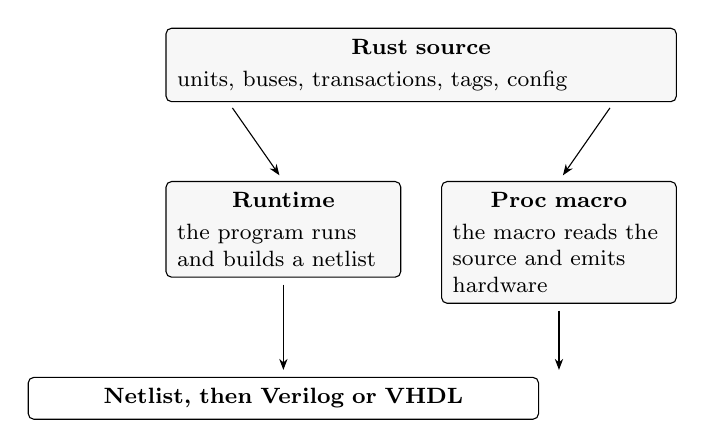
\begin{tikzpicture}[node distance=6mm]
  % Positions are computed from the boxes rather than from a fixed drop.
  % The two middle boxes have multi-line text, so a fixed `below=16mm of
  % src` put the bottom box on top of them: the build stayed green and the
  % figure was wrong.
  \node[boxf,text width=62mm,align=left] (src) {%
    \centerline{\textbf{Rust source}}\\[2pt]
    units, buses, transactions, tags, config};

  \node[boxf,text width=27mm,align=left,below=10mm of src.south west,
        anchor=north west] (rt) {%
    \centerline{\textbf{Runtime}}\\[2pt]
    the program runs and builds a netlist};

  \node[boxf,text width=27mm,align=left,below=10mm of src.south east,
        anchor=north east] (pm) {%
    \centerline{\textbf{Proc macro}}\\[2pt]
    the macro reads the source and emits hardware};

  % Below whichever of the two hangs lower.
  \node[box,text width=62mm,align=center] (out)
    at ($(src.south)!1!(rt.south |- pm.south) + (0,-12mm)$)
    {\textbf{Netlist, then Verilog or VHDL}};

  \draw[fl] (src.south west) ++(8mm,0) -- (rt.north);
  \draw[fl] (src.south east) ++(-8mm,0) -- (pm.north);
  \draw[fl] (rt.south) -- (rt.south |- out.north);
  \draw[fl] (pm.south) -- (pm.south |- out.north);
\end{tikzpicture}
\caption{The two elaboration models. Only the right-hand one can
reinterpret \code{if} on a signal, because only it sees the source.}
\label{fig:elaboration}
\end{figure}

\textbf{Runtime elaboration.} The program runs, builds a netlist through
side effects, and emits Verilog. Chisel~\cite{bachrach2012} works this way,
and for the structural half of this design it would work here unchanged.
The full expressive power of standard Rust remains available for metaprogramming
and hardware generation without requiring procedural macros. However, native
\code{if} on dynamic signals remains impossible, maintaining the constraints
detailed in Section~\ref{sec:e-walls}, and generator errors surface at execution
time rather than during compilation.

\textbf{Proc macro elaboration.} An attribute on the unit parses the item's
own source and emits hardware from it. \code{if} and \code{match} on
signals can be reinterpreted structurally, which removes
Section~\ref{sec:e-walls} entirely, and mistakes are compile errors. The
cost is real and should be stated plainly: the code looks like Rust and
does not mean Rust, and a reader who assumes Rust semantics inside a unit
will be wrong.

\begin{rulebox}[Recommendation]
Proc macro elaboration. Control flow on a signal is the largest remaining
cost of embedding, and this is the only approach that removes it.
\end{rulebox}

The second thesis' argument applies here unchanged. If a toolchain is
affordable to build, it is worth building the one that buys the most, and a
front end over Rust's syntax tree buys the type system, the module system,
the generics, the package manager and the editor tooling along with it.

\textbf{What was built.} \code{\#[lower]} is the proc macro
elaboration, with one departure from the recommendation as stated.
It reads \code{if} and \code{match} as Rust means them rather than
reinterpreting them, and reads a subset that is also plain Rust,
\code{with!}, \code{case!} and \code{select!} among registers,
wires, memories and channel ports, and refuses the rest with a message
of its own. So the cost above,
code that looks like Rust and does not mean Rust, was not paid: a
unit that lowers is the unit that simulates, one file, and the
runtime~\cite{runtime} and examples~\cite{examples} documents state
what the subset is and check every piece of it against a trace under
\code{nvc}. The RISC-V core~\cite{vreteno} is written in that subset
whole. A function under \code{\#[lower]} is the one addition since:
combinational, a few \code{let}s and a value, plain Rust for the
simulation and inlined at every call in a lowered unit of the same
file. The macro reads the file for it, which
\code{Span::local\_file} names, since a proc macro sees one item at
a time. So a step can be short and its pieces named; the core's
serial port is written so.

% SPDX-License-Identifier: Apache-2.0
\section{Related Work}
\label{sec:e-related}

Three systems bound this design, and it is closer to each than to the
others.

\textbf{Chisel}~\cite{bachrach2012} is the structural half. A hardware
module is a class in a general-purpose language, a bundle of wires has a
direction per field through \code{Flipped}, control flow on a signal is
\code{when} and \code{Mux}, and elaboration is the program running and
recording a graph. Sections~\ref{sec:e-units} to~\ref{sec:e-binding} are
that architecture in Rust, and they should be read as a port rather than
a proposal. SpinalHDL follows the same shape in the same host language.
Two things differ, both because of the host. Rust's ownership makes a
second driver on a wire a move error at compile time, where Chisel
detects it at elaboration. And Rust's trait system lets a configuration be
a type, so a build is a type alias and a binding path cannot go stale.

\textbf{Calyx}~\cite{calyx} is the nearest ancestor of the behavioural
half, and it is an intermediate representation rather than a language.
It separates structure, the wires and groups that compute, from control,
a program that says when groups run. Its control has \code{seq}, which
runs groups one after another, and \code{par}, which runs them at once.
Section~\ref{sec:e-units} arrives at the same two operators from the other
direction: an \code{await} is a \code{seq} boundary, and
\code{parallel!} is \code{par}. Calyx lowers both to a state machine
driving the groups; this paper's lowering, Section~\ref{sec:e-next},
reads a loop of one wait and lowers it to a module, and a loop of
several waits to a state machine with a state per wait, which is
Calyx's control program in its plainest form, a \code{seq} of groups,
with a wait under \code{if} the branch in it and a \code{for} that
waits a counted loop, its turns kept in a register.

\textbf{Filament}~\cite{filament} types each signal with the interval of
cycles over which it is valid, so that composing two components with
different latencies is checked rather than simulated. That is what an
\code{async} operator whose latency the mapping decides is reaching for.
Filament makes the latency part of the type and checks it statically;
this paper defers it to the mapping and would learn it at elaboration.
Filament's is the stronger guarantee, and the price is that latency has
to be stated in the type. Whether an \code{async fn} can be given a
timeline type after the fact is an open question.

\textbf{RHDL}~\cite{rhdl} is the nearest thing in Rust, and the source
of one decision here. It embeds a hardware description language in Rust
with the clock domain as a type parameter of the signal, so that a
crossing without a synchroniser is a type error. Section~\ref{sec:e-wiring}
takes that directly, and departs from it only in what the default domain
means. RHDL's structural model is Chisel's; its behavioural model is
Rust functions on values, evaluated to produce combinational logic, with
registers explicit. It has no \code{async}, so the sequencing half of
this paper is as far from RHDL as from Chisel.

\textbf{XLS}~\cite{xls} is the one to weigh most carefully, because it
is a working toolchain that has done what Section~\ref{sec:e-next} calls
the next experiment. Its front end, DSLX, is a dataflow language with
Rust's surface syntax: \code{fn}, \code{let}, \code{match}, structs,
enums and parametric types, read by a parser of its own. A DSLX function
is scheduled into a pipeline by the compiler, with the stage boundaries
chosen to meet a clock period rather than placed by the designer, which
is what Section~\ref{sec:e-pipeline} asks of an \code{async fn}. A DSLX
\code{proc} is a process with state and channels, sending and receiving
in a loop, which is the sequenced half of this paper under another
name. XLS emits Verilog, and it has been used in silicon.

That makes XLS the nearest ancestor of the behavioural half, nearer than
Calyx, and it also makes it the counterexample to this paper. XLS is the
path the project's second thesis~\cite{theses} chose: a new language,
shaped like Rust, with its own toolchain. The merged specification of
the companion paper~\cite{merge} is on that path. This paper leaves it,
and XLS is the standing evidence that the path it leaves works. The
argument for leaving it is therefore not that a separate language cannot
be made to lower; XLS shows it can. It is that the type system, the
module system, the generics, the package manager and the editor arrive
already written when the host is Rust itself, and that a DSLX-shaped
language has to rebuild each of them. Whether that trade is worth the
one wall of Section~\ref{sec:e-walls} is the question the next
experiment answers.

What is not near. Bluespec~\cite{nikhil2004} schedules guarded atomic
rules, which is a different model of concurrency from processes that
await. High-level synthesis from C or C++ starts from sequential code and
infers a pipeline, which is the same ambition as
Section~\ref{sec:e-pipeline}, from a language that has no way to say
where a boundary is allowed to fall.

Prior work on lowering coroutines or \code{async} functions to hardware
exists and has not been surveyed for this paper. That is a gap, and it is
the first thing to close before Section~\ref{sec:e-next} is attempted,
because somebody may already have found where it breaks.

\section{What Comes Next}
\label{sec:e-next}

The probes prove that the design type-checks. Chisel is a working
compiler with a decade of use. The gap between those two facts is the
whole of what remains, and it should be closed in one place rather than
widened with more probes.

\subsection{The experiment}

Lower one function to a netlist.

\begin{lstlisting}[caption={The function to lower. Two operators, two awaits, one value live across a boundary.},label={lst:next-mac}]
async fn mac(a: U<32>, b: U<32>, prev: U<64>) -> U<64> {
    let p = mul(a, b).await;
    add(prev, p).await
}
\end{lstlisting}

The lowering has to produce, from that source and nothing else, a
two-stage pipeline in Verilog: a multiplier, a register holding \code{p}
across the boundary, an adder, and a valid signal that follows the data
through. It has to do so twice, once with \code{mul} bound to a
three-cycle implementation and once to a single-cycle one, and the second
netlist has to have one register fewer than the first without any edit to
Listing~\ref{lst:next-mac}.

This test operationalizes the architectural thesis of
Section~\ref{sec:e-pipeline}. Successfully synthesizing both configurations
demonstrates that high-level procedural async definitions lower into retimed
physical pipelines. If this property cannot be verified, the framework
reduces to a structural DSL in Rust with enhanced diagnostics, rather than
achieving its intended behavioral synthesis objective.

\subsection{What it needs}

A procedural macro on the function that reads its body as a syntax tree,
finds the awaits, and splits the body at each one into a stage. The
locals live across each split are the registers. The operators awaited
are instances whose latency is looked up in the configuration. The result
is a graph, and emitting Verilog from a graph is the part Chisel has
already shown to be routine.

Three things are known to be hard, and the experiment should be designed
to meet them rather than to avoid them.

\begin{itemize}
  \item \term{Control flow across an await.} A \code{with!} whose arms
        contain awaits is a pipeline whose stages are conditional. Calyx
        handles this with \code{if} in the control program; the lowering
        needs an equivalent, and it is the first place the async model
        might not fit.
  \item \term{Resource sharing.} Section~\ref{sec:e-pipeline} claims that
        concurrent invocations at the same await index share one
        operator. The lowering has to actually do that, or the claim is
        withdrawn.
  \item \term{Backpressure.} A stage that cannot proceed is an await that
        has not completed. The valid signal has to run backwards as well
        as forwards for that to be true in hardware, which is the elastic
        pipeline of Carloni~\cite{carloni2001}, and it has to be generated
        rather than assumed.
\end{itemize}

Since this section was first written the runtime has gained a
waveform: a probe registry named from the fields of units and a VCD
writer, so a design is watched in Surfer rather than in printed
traces, and an FST writer over the same probes, the project's first
external crate. The same walk now writes a
structural netlist as well, a Verilog skeleton with modules,
registers, ports and wires and no behaviour; it sees fields only, so a
unit that takes its ports as parameters of \code{run} shows its
registers and nothing else. That gap is the argument for the
proc-macro route restated from the other side: the structure is
already recoverable at run time, and the behaviour is not.

The experiment below has since been run, in its first form. A
\code{\#[pipeline(mul = 1, add = 1)]} attribute keeps an \code{async
fn} as written and emits its Verilog beside it, each awaited operator
a stage of the stated latency and each early value delayed to meet
the operator that uses it. The same \code{mac} with \code{mul = 1}
is two stages with \code{c} delayed once; with \code{mul = 3} it is
four stages with \code{c} delayed three times; the source of the two is
identical, and the function still runs in simulation. That answers the
experiment's main question, for a grammar of awaited operator calls,
and not all of it: neither netlist has a valid signal, and the faster
one has four registers fewer than the slower, three against seven,
where the experiment asked for one fewer. A unit with state lowers
as well: \code{\#[lower]} reads a \code{run} loop of one edge wait,
register reads, \code{with!} and drives, and the blinky comes out
as a module per build, its periods baked in from the configuration;
\code{case!} lowers to a chain of comparisons with each variant's
literal, and a channel to a valid/ready handshake whose wait guards
the drives. And the lowering is checked: the same statements render to
VHDL, a testbench generated from the Rust trace replays it into the
entity under \code{nvc}, and the counter, the blinky, the sequencer,
an ALU, a scratchpad, an immediate decoder and a stage between two
channels agree with their
traces at every tick, while a deliberately broken one fails. Memories
lower, and the runtime's channel is an elastic buffer with the
handshake registered on both sides, which is the backpressure of the
list above made real rather than assumed, so a unit with channels is
checked as any other. The largest thing lowered is a three-stage RV32IMAC
core~\cite{vreteno}, written in the subset the lowering reads,
checked in lockstep against a reference model and, as a netlist,
against its own trace, placed and routed at 100~MHz on an Artix-7,
and run on the board, where it said what its simulation said; and a
unit's processes are its loops, on either edge, each a
clocked block of its own; and a loop of several waits is a state
machine, its register numbered by the lowering, so a protocol of
several steps is written as the steps rather than as a machine by
hand. Of the three things known to be hard, control flow across an
await is done, for a plain sequence, a loop of a constant count and a
wait under \code{if}, and resource sharing remains.

\subsection{What it does not need}

A parser, a type checker, a module system, generics, a package manager or
an editor. That list is the argument for embedding, and it is why the
experiment is a macro of a few hundred lines rather than a compiler.

% SPDX-License-Identifier: Apache-2.0
\section{Conclusion}
\label{sec:e-conclusion}

A companion paper merged two hardware description languages into one with
Rust-like syntax. This paper evaluated removing every construct Rust natively
provides to determine the minimal viable embedded subset.

Seventeen of twenty domain-specific constructs were eliminated, reducing the
language from a distinct grammar to four core Rust modules and procedural macros.

Two design simplifications proved especially significant. First, timeless dataflow
cannot count cycles because cycle counting requires \code{.await}, making
retiming invariants enforceable directly through Rust's type system rather than
specialized compiler checks. Second, pipelines, transaction sequences, and
concurrent processes represent a single construct (\code{async fn}) differentiated
solely by execution drivers; async state machine synthesis replaces dedicated
pipeline live-range tracking.

Two negative experimental findings guided the architecture. Arbitrary-width
arithmetic requires nightly compiler features due to const-eval limits. Furthermore,
concurrent processes cannot hold simultaneous mutable borrows of unit state;
modeling registers via interior mutability cells provides a cleaner abstraction
for shared hardware state.

To support dynamic signal selection without separate grammar parsing, the
runtime provides \code{with!}, \code{case!}, and \code{select!} macros that
lower directly into priority multiplexer trees.

While the structural features of this architecture transpose Chisel's
proven concepts into Rust with stronger static typing, the primary contribution
is unifying hardware pipelines and protocols through \code{async fn}. As
demonstrated by lowering a verified RV32I core~\cite{vreteno} at 100~MHz on
FPGA hardware, embedding TxHDL within Rust harnesses an industrial-grade type
system while concentrating design effort on novel behavioral synthesis.


\begin{thebibliography}{10}

\bibitem{merge}
F.~Filmar and D.~Janković, ``TxHDL: Unifying a dataflow and a transaction
hardware description language,'' project repository \code{HDL/txhdl},
\code{docs/article.tex}, 2026.

\bibitem{unification}
``Unifying LHDL and TxHDL,'' project repository \code{HDL/txhdl},
\code{docs/unification-analysis.md}, 2026. States what each source language
contributes and resolves the four conflicts of meaning.

\bibitem{syntax}
``Surface syntax for the merged language,'' project repository
\code{HDL/txhdl}, \code{docs/syntax-decisions.md}, 2026. Settles the
spelling of every construct, biased toward Rust.

\bibitem{theses}
F.~Filmar, ``Some theses for a modern hardware definition language,''
project repository \code{HDL/txhdl}, \code{filmil/theses.md}, 2026.

\bibitem{embedding}
``Embedding TxHDL in Rust,'' project repository \code{HDL/txhdl},
\code{docs/rust-embedding.md}, 2026. The working notes this article is
drawn from, with the probe results in full.

\bibitem{build}
``Building the specification documents,'' project repository
\code{HDL/txhdl}, \code{docs/document-build-plan.md}, 2026.

\bibitem{runtime}
F.~Filmar and D.~Janković, ``The TxHDL runtime,'' project repository
\code{HDL/txhdl}, \code{//docs:runtime}, 2026. The library, included
verbatim, with the model of time it implements.

\bibitem{examples}
F.~Filmar and D.~Janković, ``TxHDL by example,'' project repository
\code{HDL/txhdl}, \code{//docs:examples}, 2026. One compiled example
per concept, with its output where it has one.

\bibitem{vreteno}
F.~Filmar and D.~Janković, ``Vreteno: An RV32I core in TxHDL,''
project repository \code{HDL/txhdl}, \code{//docs:vreteno}, 2026.

\bibitem{cover}
F.~Filmar and D.~Janković, ``TxHDL documents,'' project repository
\code{HDL/txhdl}, \code{//docs:cover}, 2026.

\bibitem{bachrach2012}
J.~Bachrach \emph{et al.}, ``Chisel: Constructing hardware in a Scala
embedded language,'' in \emph{Proc. Design Automation Conf.}, 2012, pp.
1216--1225.

\bibitem{calyx}
R.~Nigam, S.~Thomas, Z.~Li, and A.~Sampson, ``A compiler infrastructure
for accelerator generators,'' in \emph{Proc. ASPLOS}, 2021, pp. 804--817.

\bibitem{filament}
R.~Nigam, P.~Kumar, and A.~Sampson, ``Modular hardware design with
timeline types,'' \emph{Proc. ACM Program. Lang.}, vol.~7, no. PLDI, 2023.

\bibitem{xls}
Google, ``XLS: Accelerated hardware synthesis,'' software,
\code{https://github.com/google/xls}, 2020 onwards. DSLX is its front
end.

\bibitem{rhdl}
S.~Basu, ``RHDL: a hardware description language embedded in Rust,''
software, \code{https://github.com/samitbasu/rhdl}, 2023 onwards.

\bibitem{nikhil2004}
R.~Nikhil, ``Bluespec System Verilog: efficient, correct RTL from high level
specifications,'' in \emph{Proc. MEMOCODE}, 2004, pp. 69--70.

\bibitem{carloni2001}
L.~P. Carloni, K.~L. McMillan, and A.~L. Sangiovanni-Vincentelli, ``Theory
of latency-insensitive design,'' \emph{IEEE Trans. Computer-Aided Design},
vol.~20, no.~9, pp. 1059--1076, 2001.

\bibitem{rust}
N.~D. Matsakis and F.~S. Klock, ``The Rust language,'' \emph{Ada Letters},
vol.~34, no.~3, pp. 103--104, 2014.

\end{thebibliography}

\end{document}
